\section{Results}

\subsection{Traits and diversification}

When analyzed separately, ploidy and breeding system each showed significant associations with net diversification differences in Solanaceae.
When analyzed together, however, the effect of breeding system dominated the effect of ploidy, although hidden factors played an important role as well.

When considering ploidy alone ($D/P$ model), we found a greater net diversification rate for diploids than for polyploids, in agreement with \citet{mayrose_2011, mayrose_2015}.
This result holds with (\cref{figure:netdivall}A) or without (\cref{figure:netdivnodip}A) the diploidization parameter, although including diploidization shifts the net diversification rate of polyploids to be non-negative.
Incorporating a hidden state in this model, however, reduces the clear separation in diversification rate estimates between diploids and polyploids ($D/P+A/B$ model; \cref{figure:netdivall}B, \cref{figure:netdivnodip}B).
Thus, differences in net diversification rates are explained by an unknown factor as well as by ploidy.
% E: I edited the interpretation of D/P+A/B.  There still is some separation between D/P within each A/B.  The A/B separation isn't any clearer, at least.
Statistical model comparisons show very strong support for including the hidden state and strong support for including diploidization (\cref{table:bayesfactors}).

When considering breeding system alone ($I/C$ model, \cref{figure:netdivall}C), we found a larger net diversification rate for SI than for SC species, in agreement with \citet{goldberg_2010}.
When a hidden state is included ($I/C+A/B$ model), the large net diversification rate difference persists for one of the hidden states but is mostly removed for the other (\cref{figure:netdivall}D).
Thus, differences in net diversification rates are best explained by both breeding system and an unknown factor \citep[as in Onagraceae;][]{freyman_2019}.
% The transition rate from SI to SC is $q_{IC}=0.3$ for both the I/C and the I/C+A/B models.
The statistical model comparison shows very strong support for including the hidden state (\cref{table:bayesfactors}).

When considering ploidy and breeding system together ($ID/CD/CP$ model), the net diversification rate for SI diploids was greater than for either SC diploids or SC polyploids, with or without diploidization (\cref{figure:netdivall}E, \cref{figure:netdivnodip}C).
Thus, the difference in net diversification associated with breeding system persists even when ploidy is included in the model.
The reverse is not true, though: the association of ploidy with net diversification in the $D/P$ model (\cref{figure:netdivall}A, \cref{figure:netdivnodip}A) appears to be driven by the subset of diploids that are SI; among SC species, net diversification rates for diploids and polyploids not as distinct.
%
When a hidden state is included ($IC/CD/CP+A/B$ model), the same general pattern remains when diploidization is prevented (\cref{figure:netdivnodip}D), although the higher net diversification rate of $ID$ is less clear within one of the hidden states.
With diploidization, the net diversification rate of $ID$ is still greater than $CD$ within each hidden state, but diversification estimate for $CP$ is highly uncertain and perhaps bimodal.
Statistical model comparisons show very strong support for including the hidden state and at most positive support for including diploidization (\cref{table:bayesfactors}).

\subsection{Pathways to polyploidy}

There are two pathways by which SI diploid lineages eventually---given enough time---become SC polyploids.
In the one-step pathway, polyploidization directly disables SI.
In the two-step pathway, SI is first lost within the diploid state, followed by polyploidization.
Determining the relative contribution of these pathways based on our estimated transition rates from the $ID/CD/CP$ model, we find that the one-step pathway is more likely on short timescales and the two-step pathway is more likely on long timescales (\cref{figure:pathways}, left panels).
Beginning with a single SI diploid lineage, when not much time has elapsed, the one-step pathway is more likely because it only necessitates a single event to effect transition to the SC polyploid state.
When more time has elapsed, the two-step pathway is more likely because the rate of loss of SI within diploids, $q_{IC}$, is greater than the rate of polyploidization for SI species, $\rho_I$ (\cref{suppfigure:IDCDCPnodip}).
That is, an $ID$ lineage is more likely to begin its path to polyploidy with a transition to $CD$, but completing this path to $CP$ takes longer.

The preceding conclusions, however, ignore the changes in numbers of lineages in each state due to speciation and extinction.
By analogy, envisioning the states as stepping stones, the extent to which each stone grows or shrinks over time affects the utility of each possible path.
Allowing for the different net diversification rates for each state, we find a qualitative difference in the relative pathway contributions.
In particular, the lower rate of net diversification in the $CD$ state, relative to $ID$, means that relatively fewer lineages are available to complete the second step of the two-step pathway, ending in $CP$.
Consequently, even over long timescales, the two-step pathway contributes less to the formation of polyploids (\cref{figure:pathways}, right panels).

\subsection{Diploidization as an exploratory hypothesis}

We considered models both with and without diploidization in order to explore its effects on the estimates of state-dependent diversification.
For the two models that only include diploid and polyploid states ($D/P$ and $D/P+A/B$), the net diversification rate of polyploid lineages is likely negative when diploidization (parameter $\delta$) is excluded but positive when it is included (\cref{figure:netdivall}A versus \cref{figure:netdivnodip}A).
For the two models that also included breeding system ($ID/CD/CP$ and $ID/CD/CP+A/B$), the main effect of including diploidization is greatly increasing the uncertainty of the estimated polyploid net diversification rate (\cref{figure:netdivall}EF versus \cref{figure:netdivnodip}CD).
For all models, there is greater uncertainty in the estimate of diploidization rate than polyploidization rate, as judged by the width of the credibility intervals (see \cref{suppfigure:DP,suppfigure:DPAB,suppfigure:IDCDCP,suppfigure:IDCDCPAB}).
% R will add a bit about param confidence

\begin{supptable}
    \begin{center}
    
    \begin{tabular}{lcccccc}
                       & D/P   & D/P+A/B      & I/C    & I/C+A/B      & ID/CD/CP & ID/CD/CP+A/B \\ \midrule
        %                                                                                      
        $r_D$          & 0.260 & 0.193, 0.658 & ---    & ---          & ---      & ---          \\
        $r_P$          &-0.056 & 0.030, 0.187 & ---    & ---          & ---      & ---          \\
        $r_I$          & ---   & ---          & 0.550  & 0.386, 0.877 & ---      & ---          \\
        $r_C$          & ---   & ---          &-0.001  &-0.059, 0.606 & ---      & ---          \\
        $r_{ID}$       & ---   & ---          & ---    & ---          & 0.455    & 0.309, 0.797 \\
        $r_{CD}$       & ---   & ---          & ---    & ---          & 0.065    &-0.006, 0.587 \\
        $r_{CP}$       & ---   & ---          & ---    & ---          &-0.088    &-0.074, 0.403 \\
        %                                                                                      
        $\rho$         & 0.047 & 0.047        & ---    & ---          & ---      & ---          \\
        $\rho_I$       & ---   & ---          & ---    & ---          & 0.067    & 0.053        \\
        $\rho_C$       & ---   & ---          & ---    & ---          & 0.033    & 0.032        \\
        $q_{IC}$       & ---   & ---          & 0.364  & 0.261        & 0.198    & 0.145        
    \end{tabular}
    
    \vspace{12pt}
            
    \begin{tabular}{lcccc}
                       & D/P   & D/P+A/B      & ID/CD/CP & ID/CD/CP+A/B \\ \midrule
        %                                                              
        $r_D$          & 0.382 & 0.698, 0.100 & ---      & ---          \\
        $r_P$          & 0.109 & 0.587, 0.182 & ---      & ---          \\
        $r_I$          & ---   & ---          & ---      & ---          \\
        $r_C$          & ---   & ---          & ---      & ---          \\
        $r_{ID}$       & ---   & ---          & 0.449    & 0.318, 0.789 \\
        $r_{CD}$       & ---   & ---          & 0.050    &-0.248, 0.494 \\
        $r_{CP}$       & ---   & ---          &-0.027    & 0.110, 0.634 \\
        %                                                              
        $\rho$         & 0.033 & 0.026        & ---      & ---          \\
        $\rho_I$       & ---   & ---          & 0.063    & 0.047        \\
        $\rho_C$       & ---   & ---          & 0.024    & 0.011        \\
        $\delta$       & 0.050 & 0.162        & 0.022    & 0.107        \\
        $q_{IC}$       & ---   & ---          & 0.194    & 0.164        
    \end{tabular}


    \end{center}
    \caption{
        Median rate estimates for all fitted models.
        Units are per million years.
        Two comma-separated numbers refer to the $A$ and $B$ hidden states, and --- means the parameter was not present in the model.
    Net diversification rates ($r$) are subscripted with trait state initials (Diploid, Polyploid, Incompatible, Compatible). Transition rates are $\rho$ (polyploidization), subscripted with background breeding system state; $\delta$ (diploidization); and  $q_{IC}$ (loss of self-incompatibility).
    The upper section is for models without diploidization, and the lower section is for models with diploidization.
    The supplemental figures show the corresponding distributions of parameter estimates.
    }
    \label{table:estimates}
\end{supptable}

% check values of delta and rho D/P+A/B with(out) delta
% i.e. parameter values in figure S1 & S4 vs Table S2

%B: heads up: I added two clarifying descriptive sentences in the two figures below. Maybe something about noting x-axis scale differences would be useful.
\begin{figure}
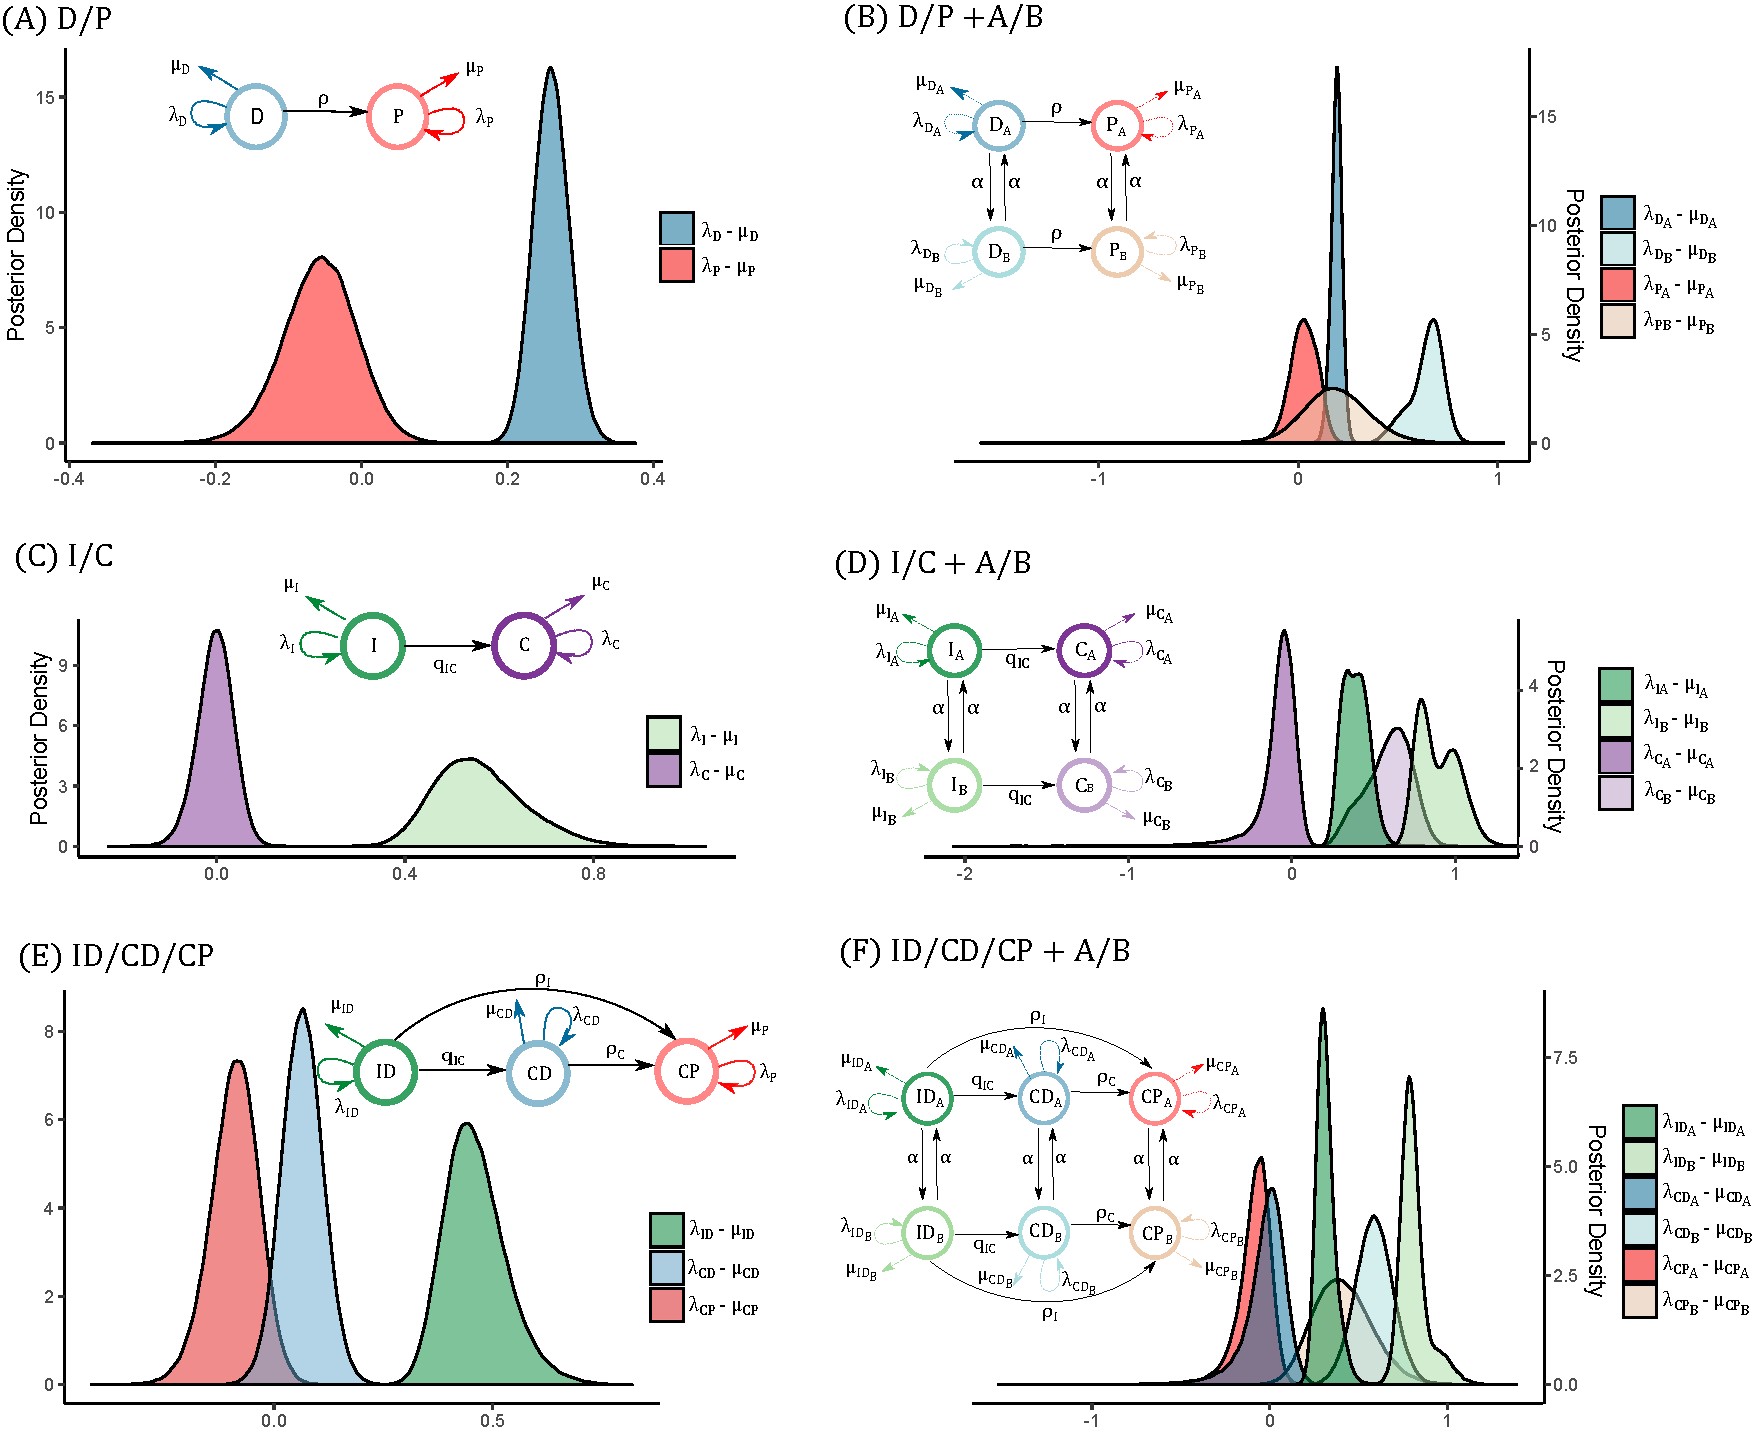
\includegraphics[width=\textwidth]{allnetdivmodelswithoutdelta.pdf} % FIXME: need horizontal axis label
\caption{Net diversification rates for all models without diploidization rate estimate. 
Each panel contains a graphical summary of estimated model parameters and displays posterior distributions for net diversification estimates.}
\label{figure:netdivall}
\end{figure}

\begin{figure}
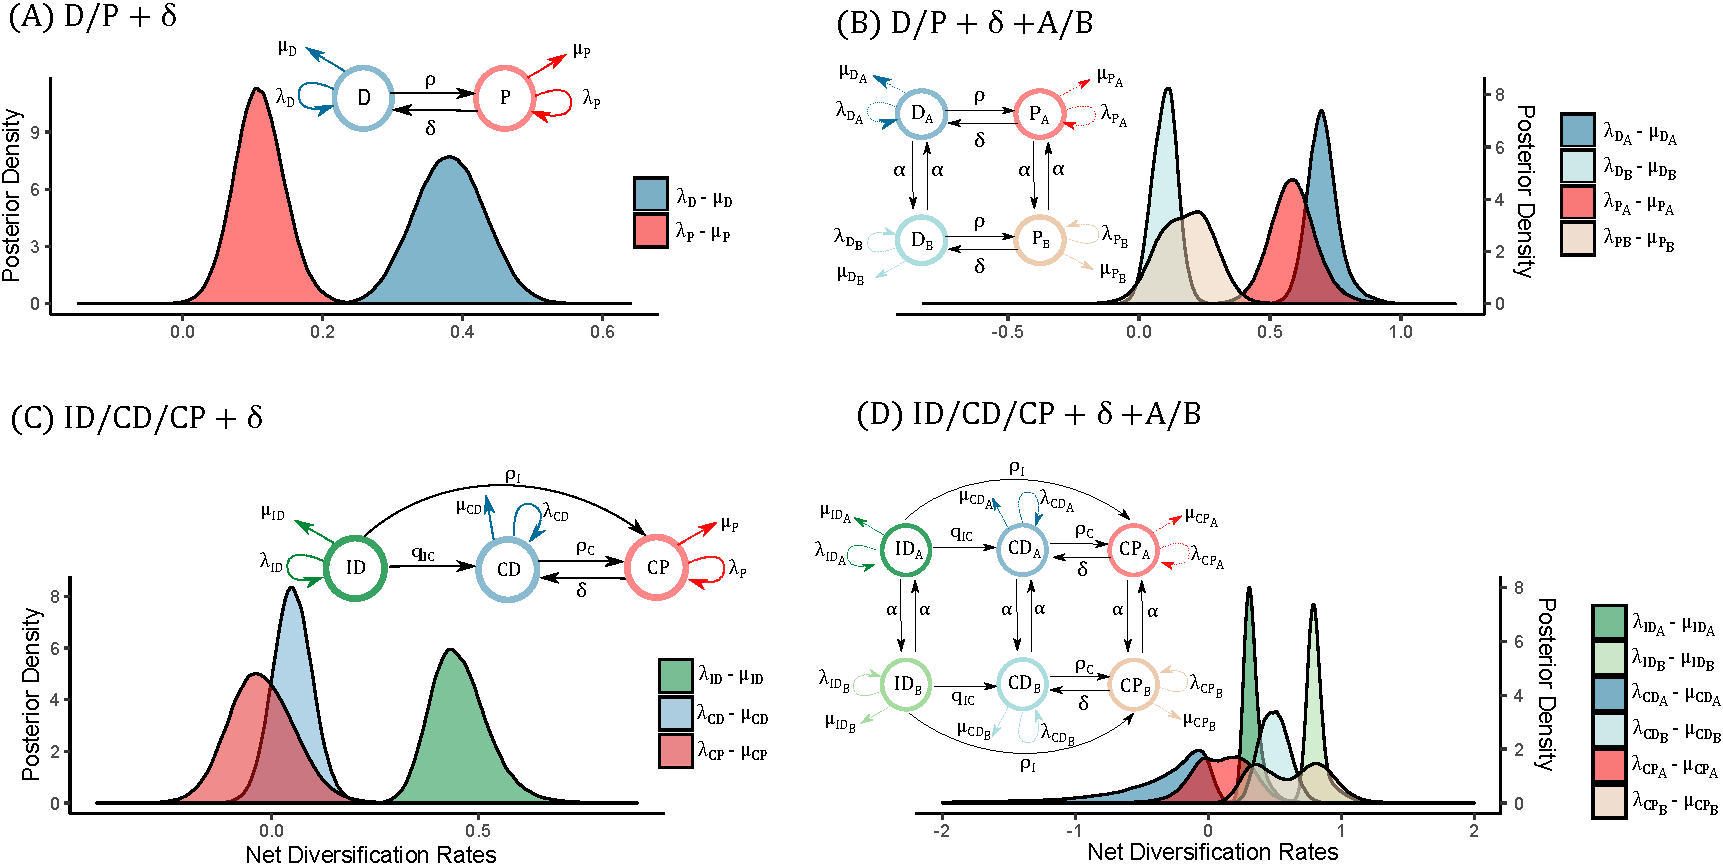
\includegraphics[width=\textwidth]{allnetdivmodelsdiploidization.pdf}
\caption{Net diversification rates for all models that include diploidization ($\delta$). 
Each panel contains a graphical summary of estimated model parameters and displays posterior distributions for net diversification estimates.}  
\label{figure:netdivnodip}
\end{figure}

% E todo: re-run with new rate estimates; add panel letters?
\begin{figure}
    \centering 
    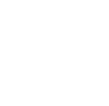
\includegraphics[width=0.5\textwidth]{pathstates} \\ [12pt]
        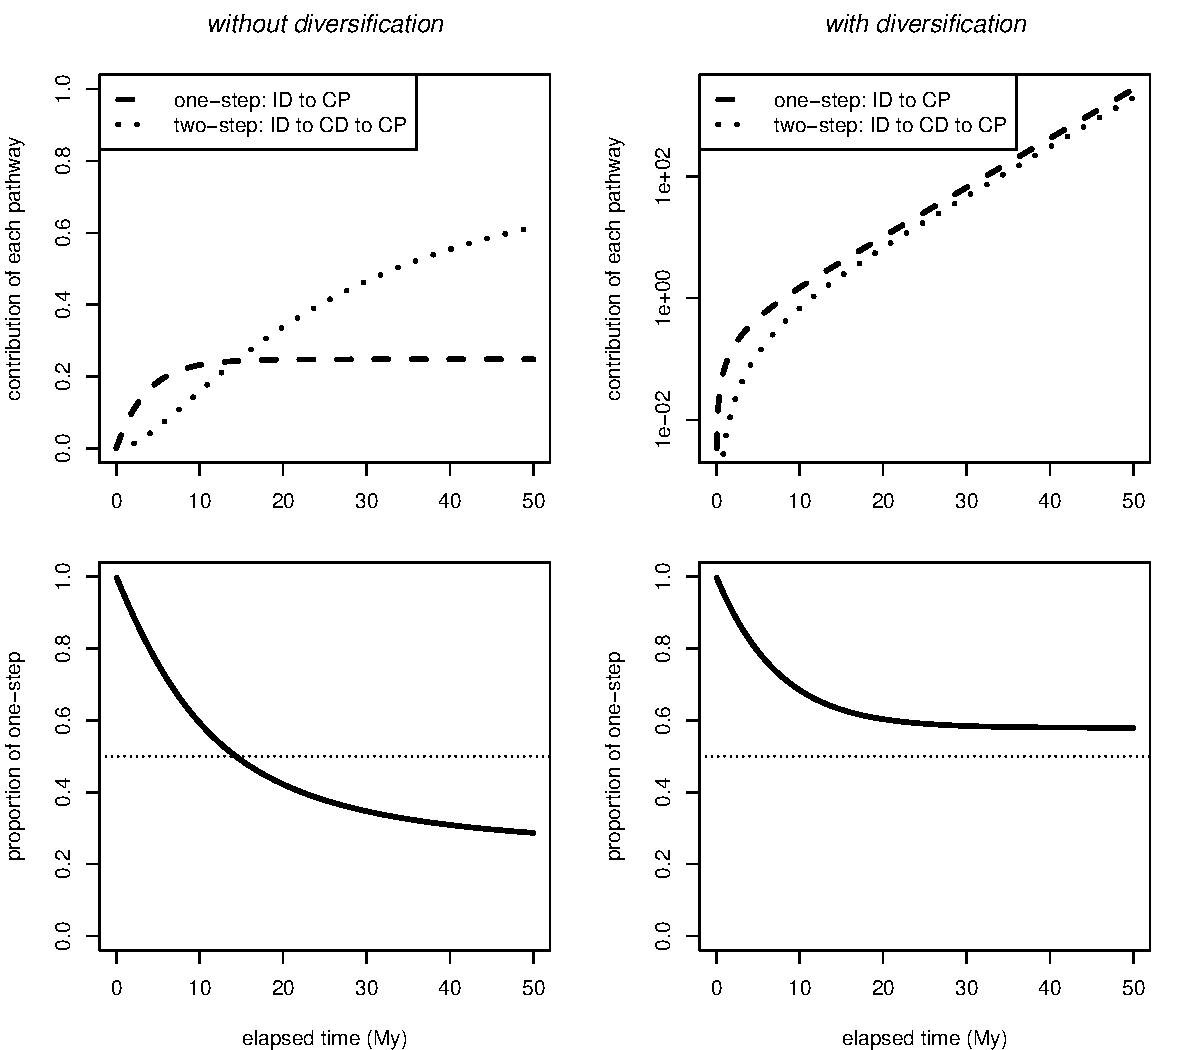
\includegraphics[width=0.9\textwidth]{pathways}
    \caption{
        Contributions of the two pathways to polyploidy.
        The one-step pathway is direct ID$\rightarrow$CP transitions.
        The two-step pathway consists of ID$\rightarrow$CD$\rightarrow$CP transitions.
        When considering only rates of transitions among the states (ignoring the diversification rate parameters), the one-step pathway dominates on short timescales and the two-step on long timescales (left panels).
        When also considering diversification within each state, the one-step pathway, in which polyploidization breaks down SI, dominates over any timescale (right panels).
        The top panels show the separate contributions of each pathway.
        The bottom panels show the proportional contribution of the one-step pathway (\ie one-step / [one-step + two-step]).
    }
    \label{figure:pathways}
\end{figure}

\begin{suppfigure}
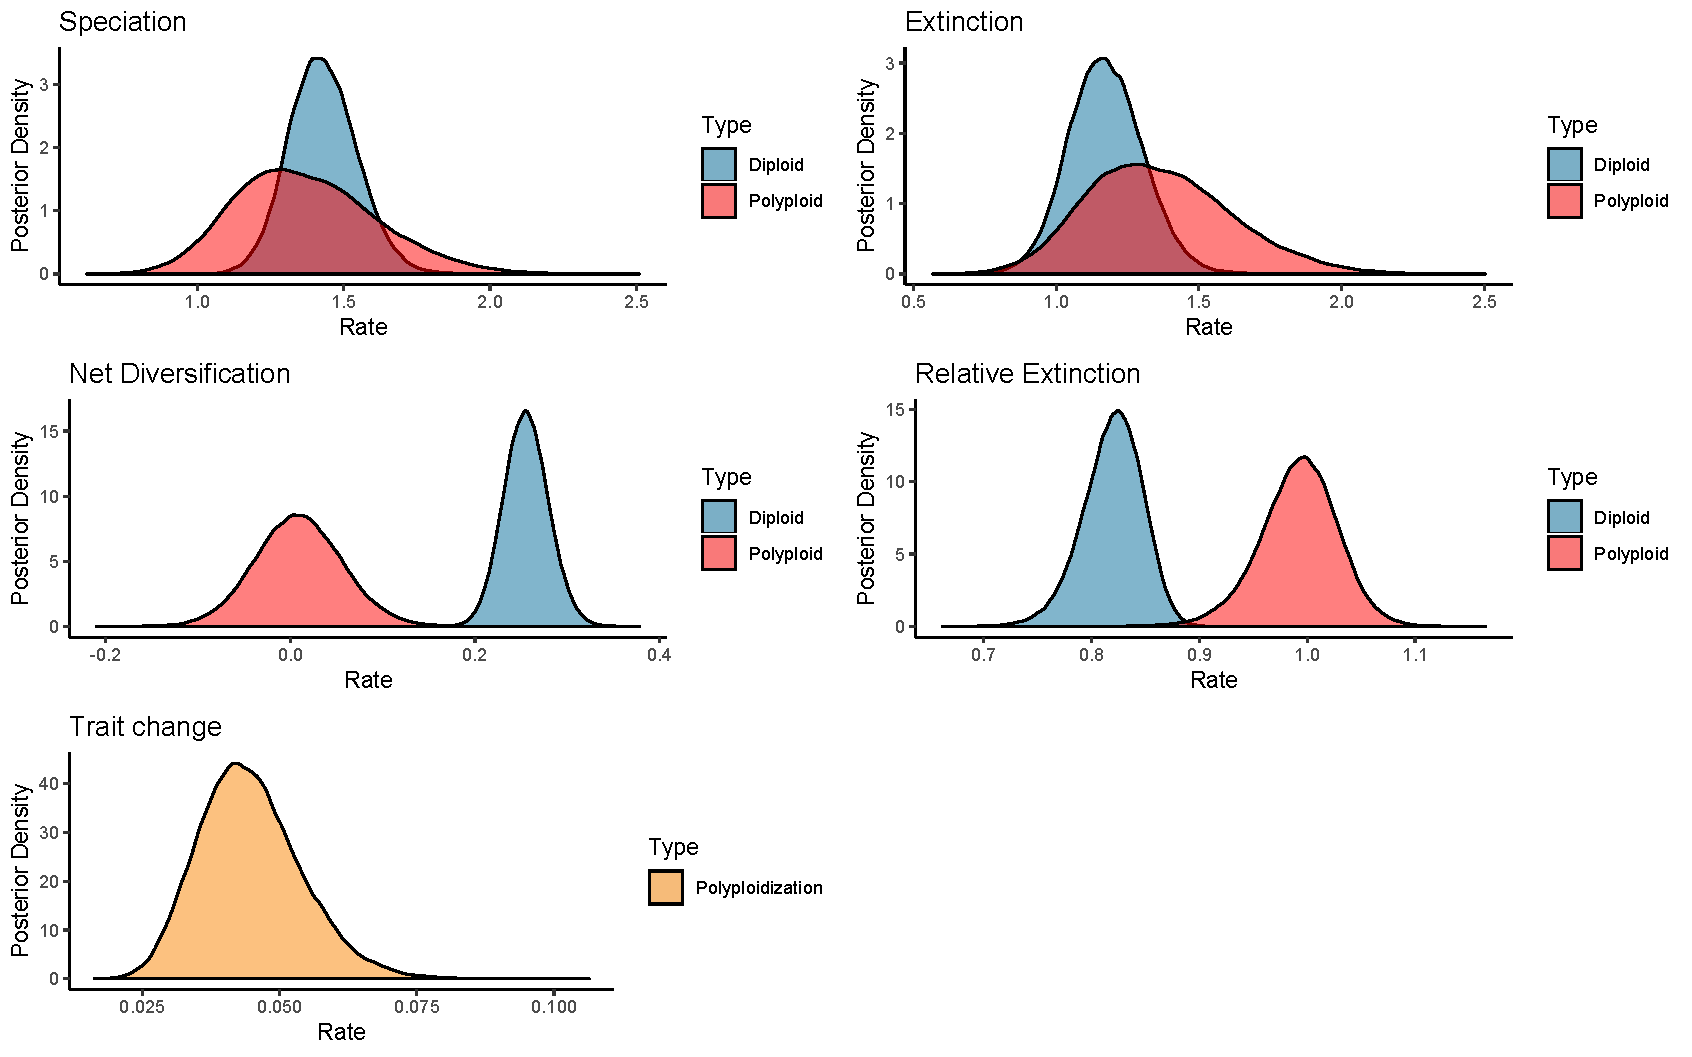
\includegraphics[width=\textwidth]{bisseDPnodipposteriordist.pdf}
\caption{Posterior distribution for each of the parameters in the D/P ploidy model} % XXX
\label{suppfigure:DPnodip}
\end{suppfigure}

\begin{suppfigure}
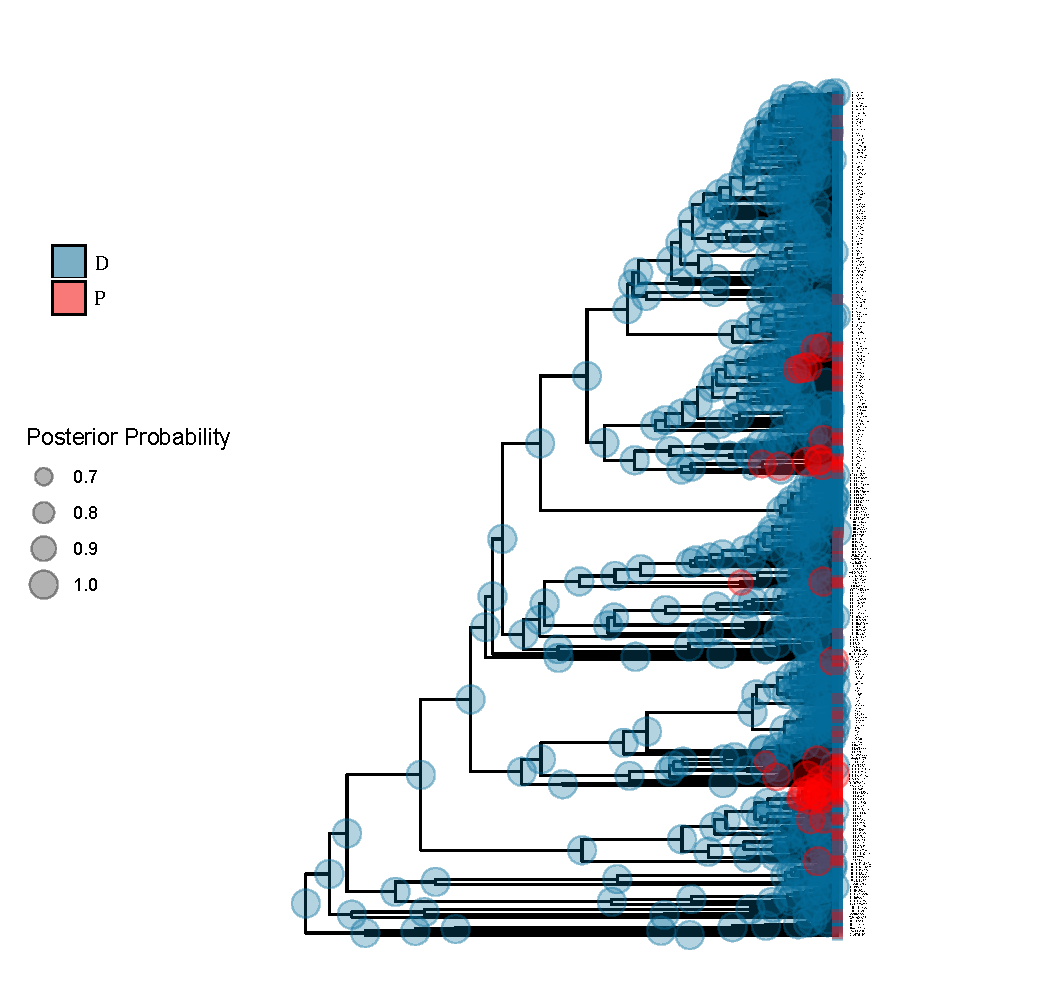
\includegraphics[width=\textwidth]{asrDP.pdf}
\caption{Ancestral state reconstruction showing the maximum a posteriori for each node of the D/P ploidy model} % XXX
\label{suppfigure:DPnodipasr}
\end{suppfigure}

\begin{suppfigure}
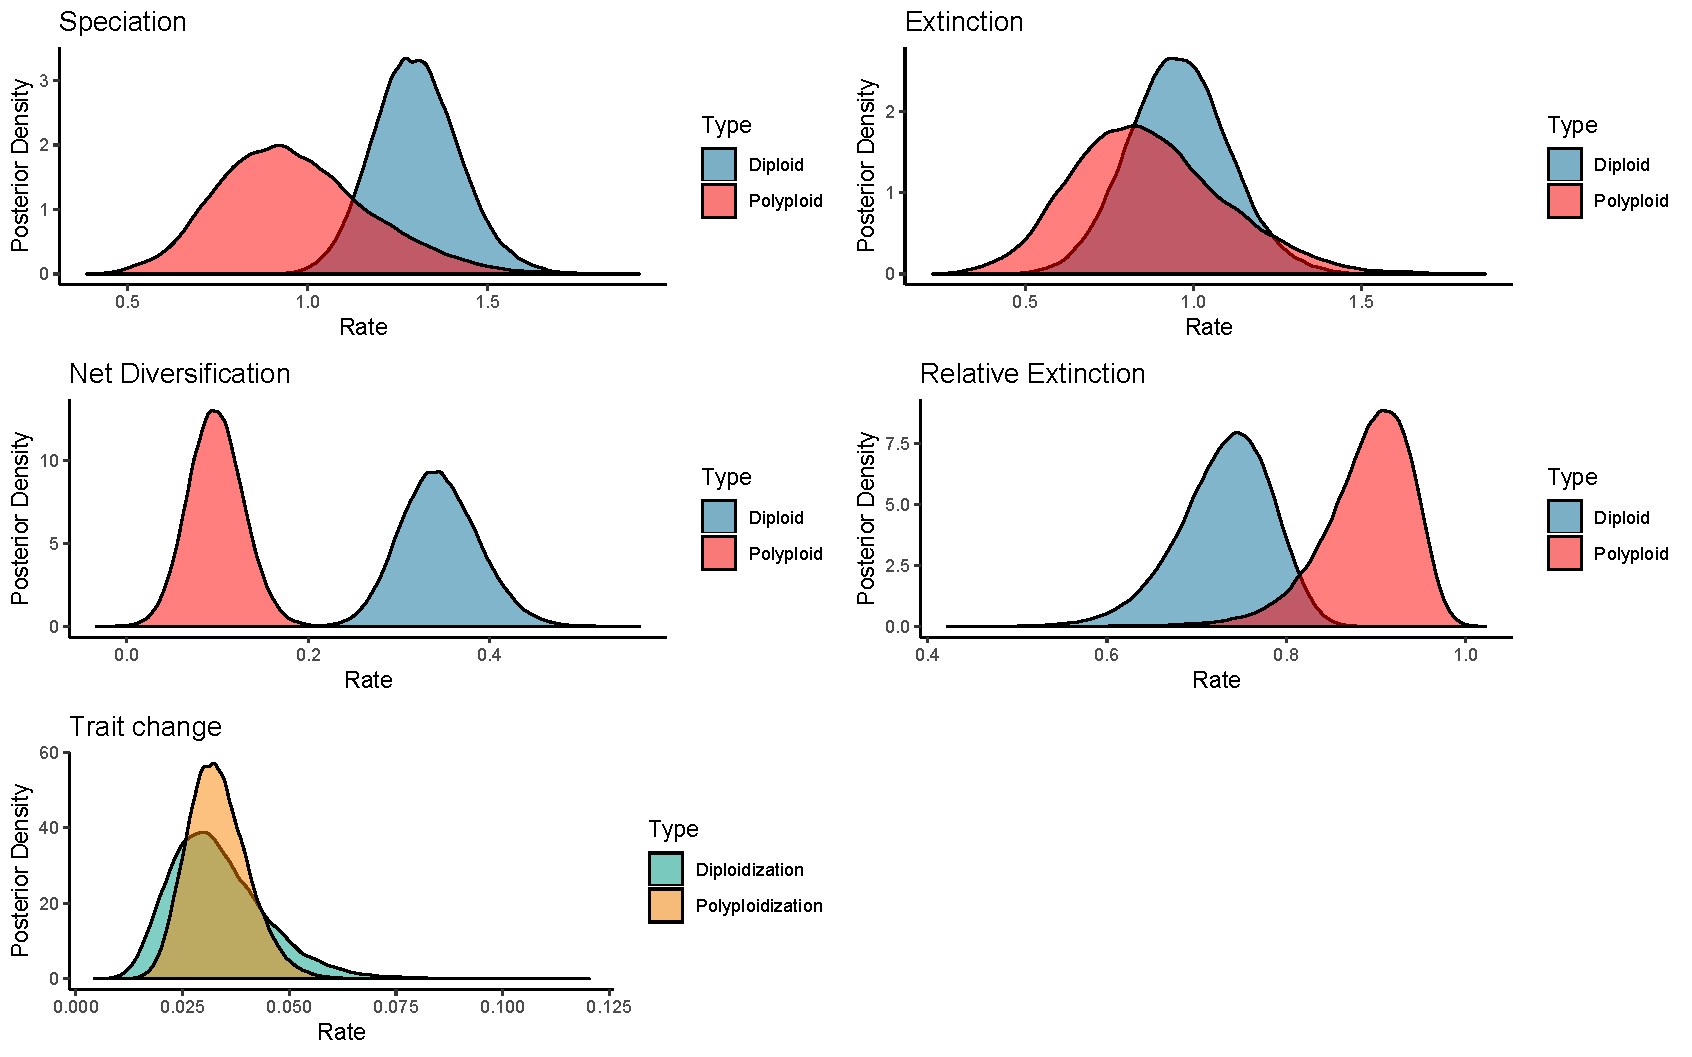
\includegraphics[width=\textwidth]{bisseDPposteriordist.pdf}
\caption{Posterior distribution for each of the parameters in the D/P+ $\delta$ ploidy model} % XXX
\label{suppfigure:DP}
\end{suppfigure}

\begin{suppfigure}
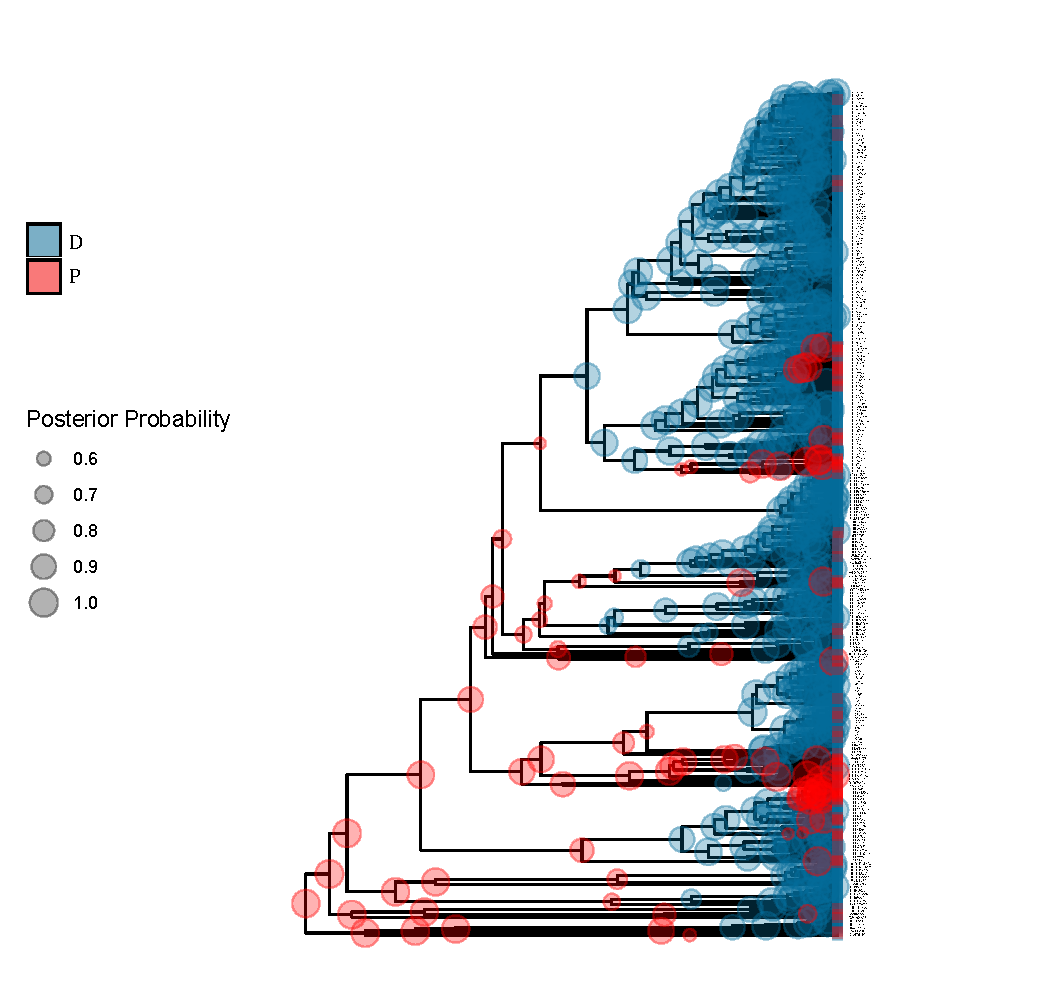
\includegraphics[width=\textwidth]{asrDPdelta.pdf}
\caption{Ancestral state reconstruction showing the maximum a posteriori for each node in the D/P+ $\delta$, ploidy model} % XXX
\label{suppfigure:DPasr}
\end{suppfigure}

\begin{suppfigure}
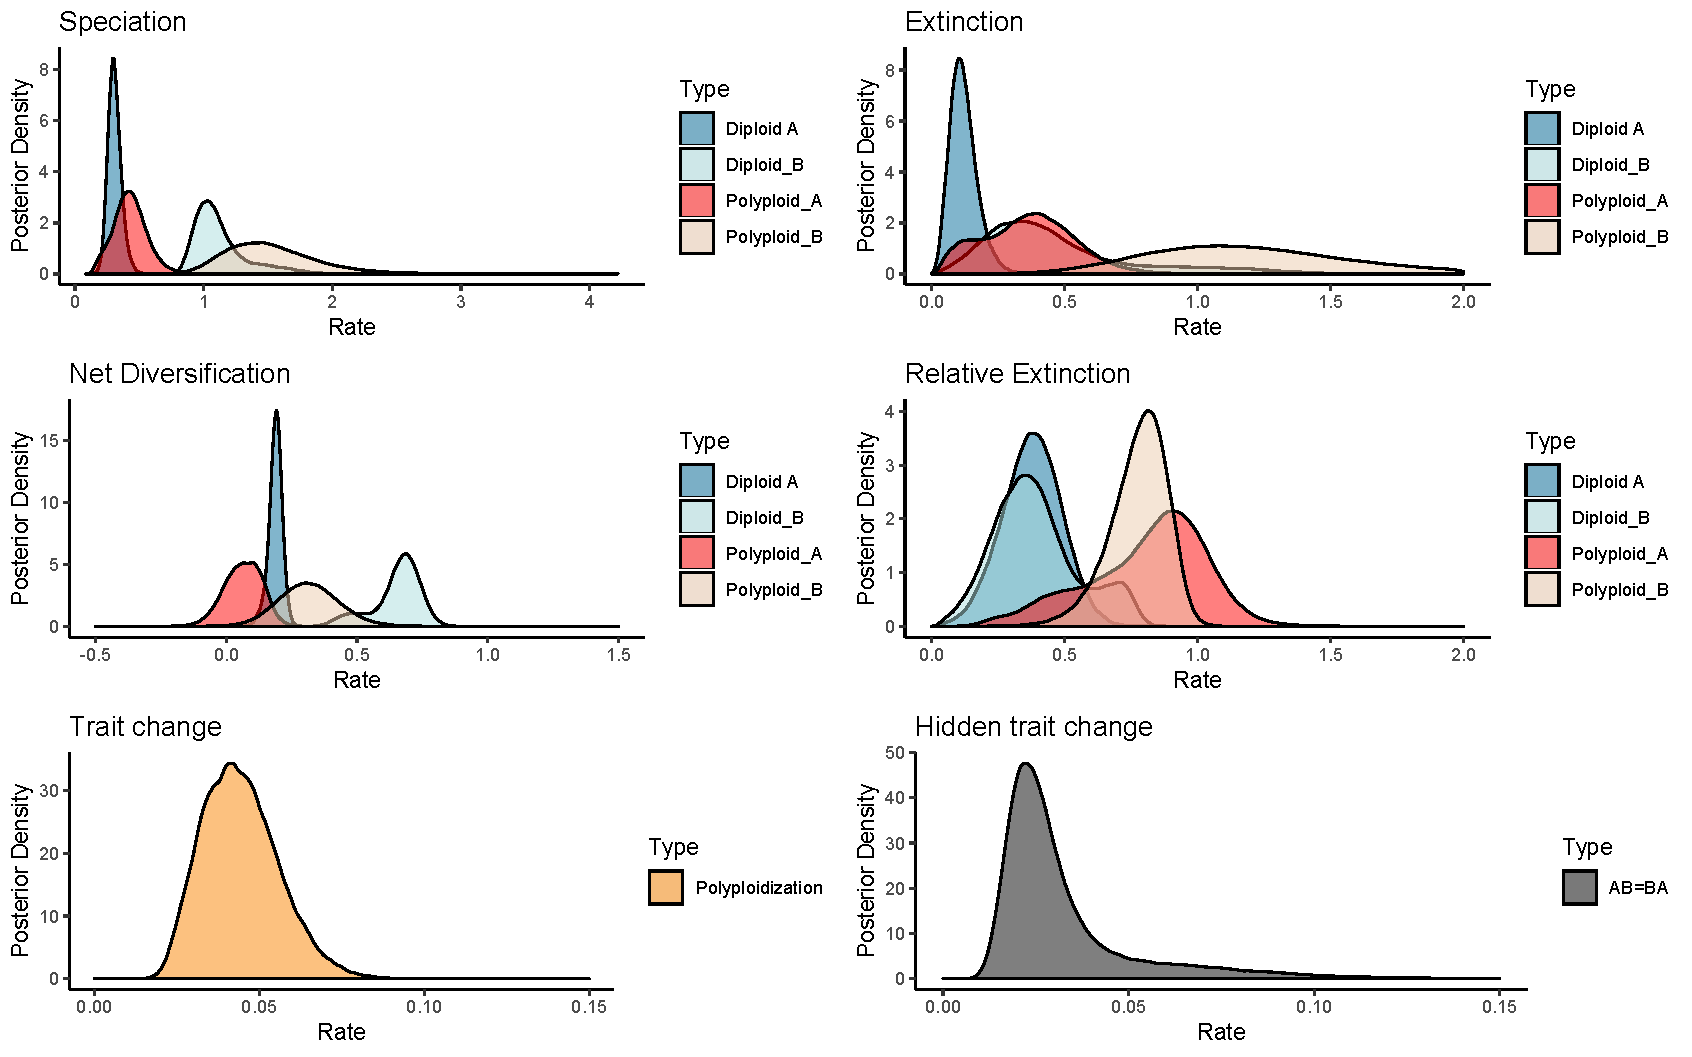
\includegraphics[width=\textwidth]{hisseDPnodipposteriordist.pdf}
\caption{Posterior distribution for each of the parameters in the D/P+A/B ploidy model} % XXX
\label{suppfigure:DPnodipAB}
\end{suppfigure}

\begin{suppfigure}
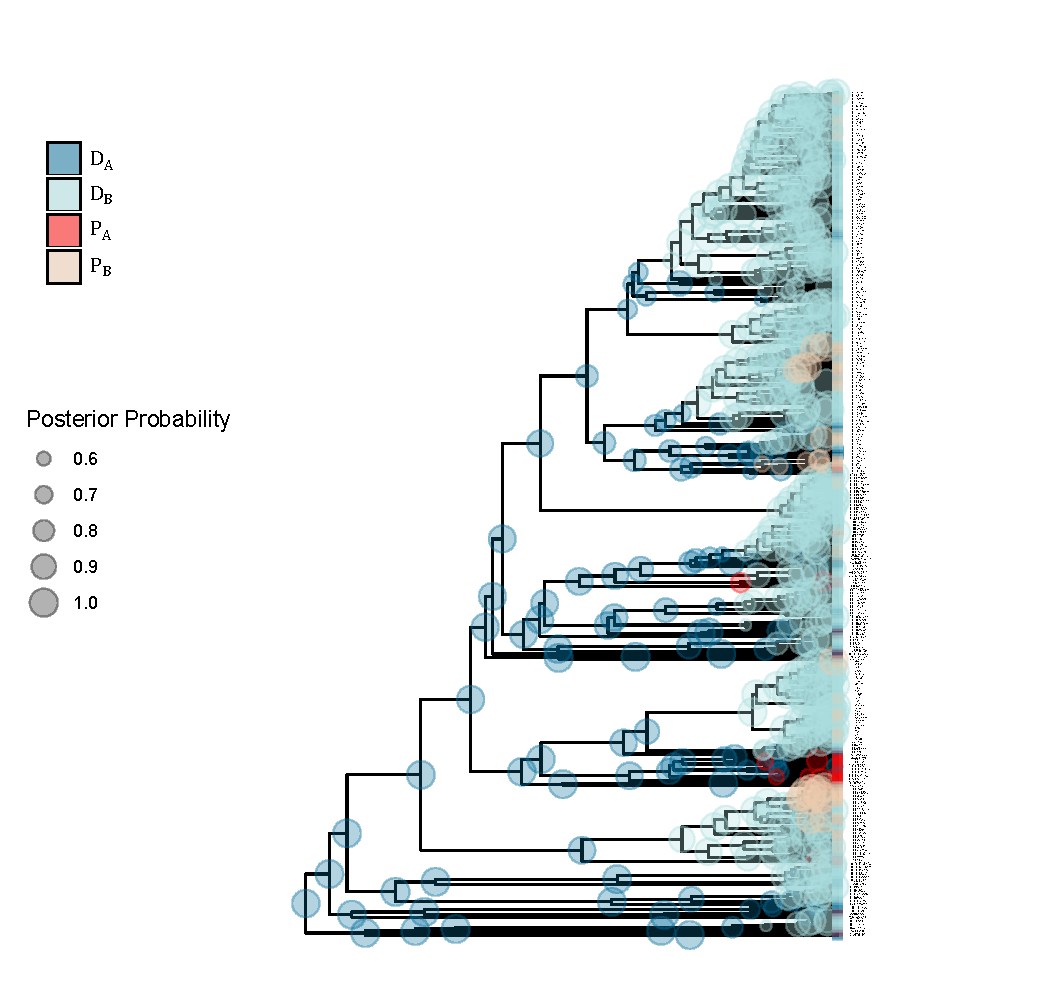
\includegraphics[width=\textwidth]{asrDPAB.pdf}
\caption{Ancestral state reconstruction showing the maximum a posteriori for each node in the D/P D/P+A/B ploidy model} % XXX
\label{suppfigure:DPnodipABasr}
\end{suppfigure}

\begin{suppfigure}
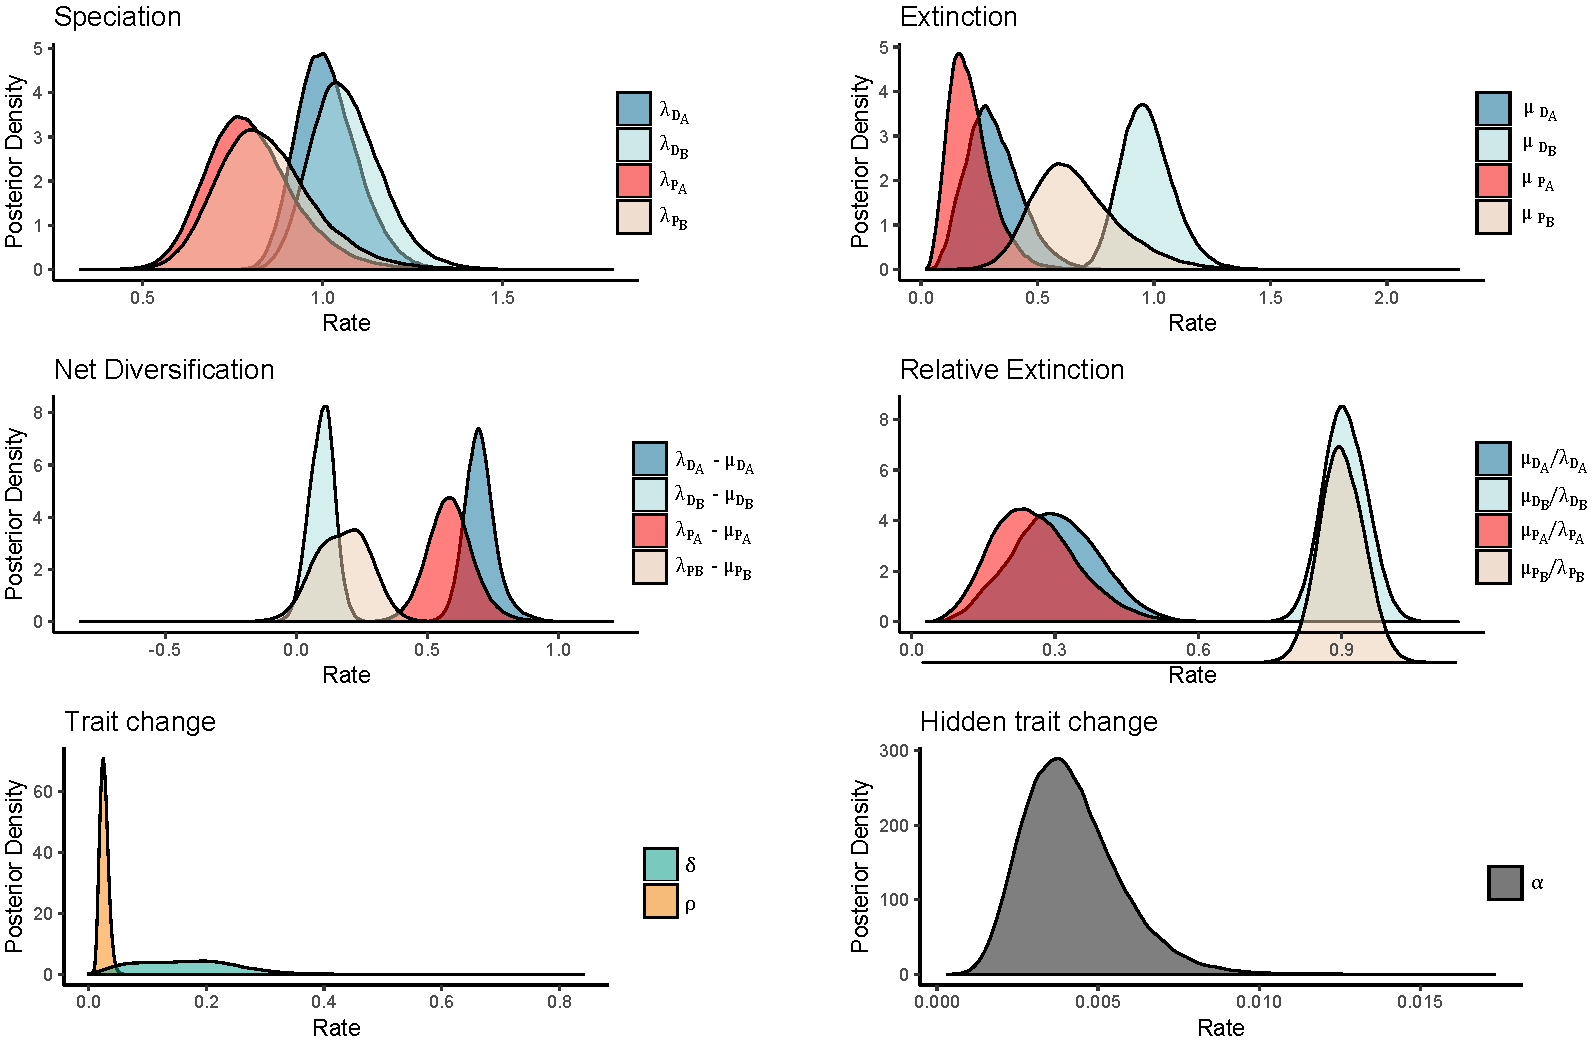
\includegraphics[width=\textwidth]{hisseDPposteriordist.pdf}
\caption{Posterior distribution for each of the parameters in the D/P+$\delta$+A/B ploidy model.  The axis is offset in one location so that the two overlapping distributions can be seen.} % XXX
\label{suppfigure:DPAB}
\end{suppfigure}

\begin{suppfigure}
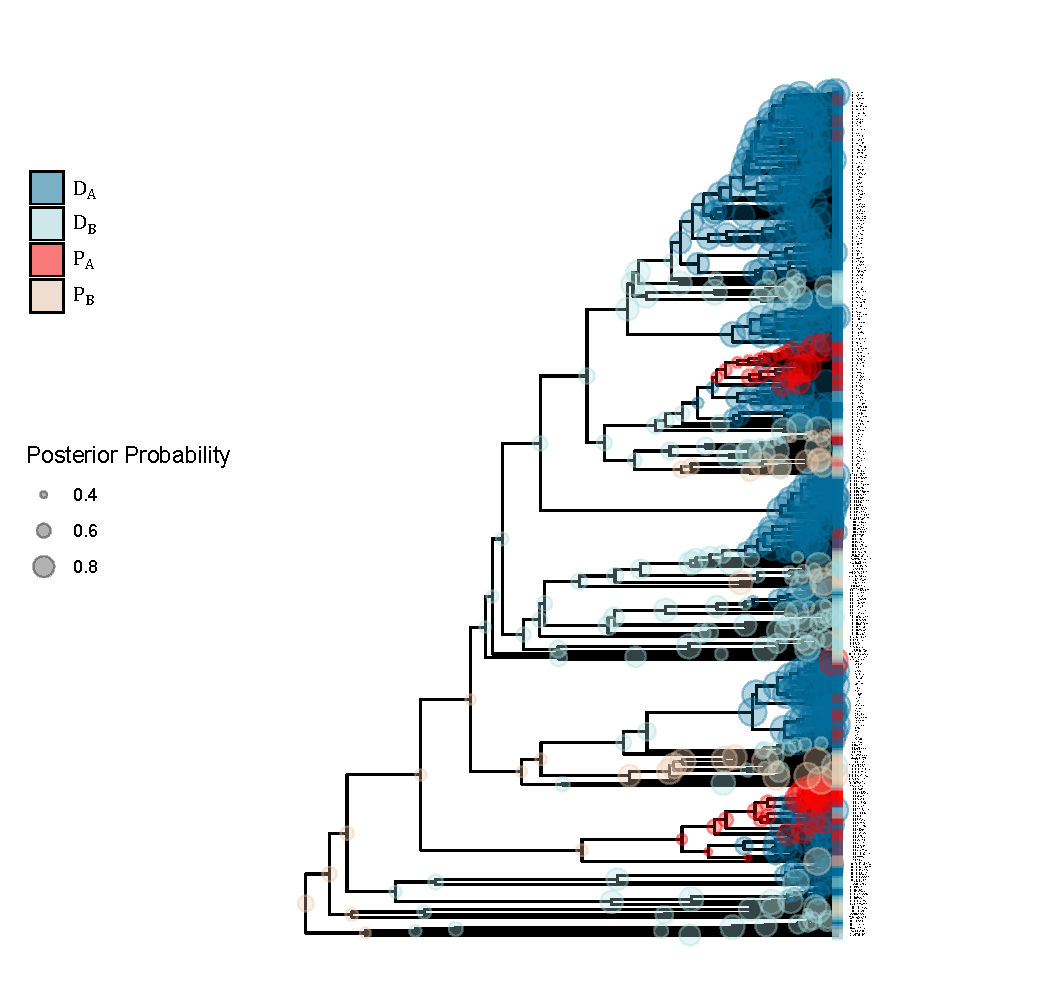
\includegraphics[width=\textwidth]{asrDPABdelta.pdf}
\caption{Ancestral state reconstruction showing the maximum a posteriori for each node in the D/P+$\delta$+A/B ploidy model.} % XXX
\label{suppfigure:DPABasr}
\end{suppfigure}

\begin{suppfigure}
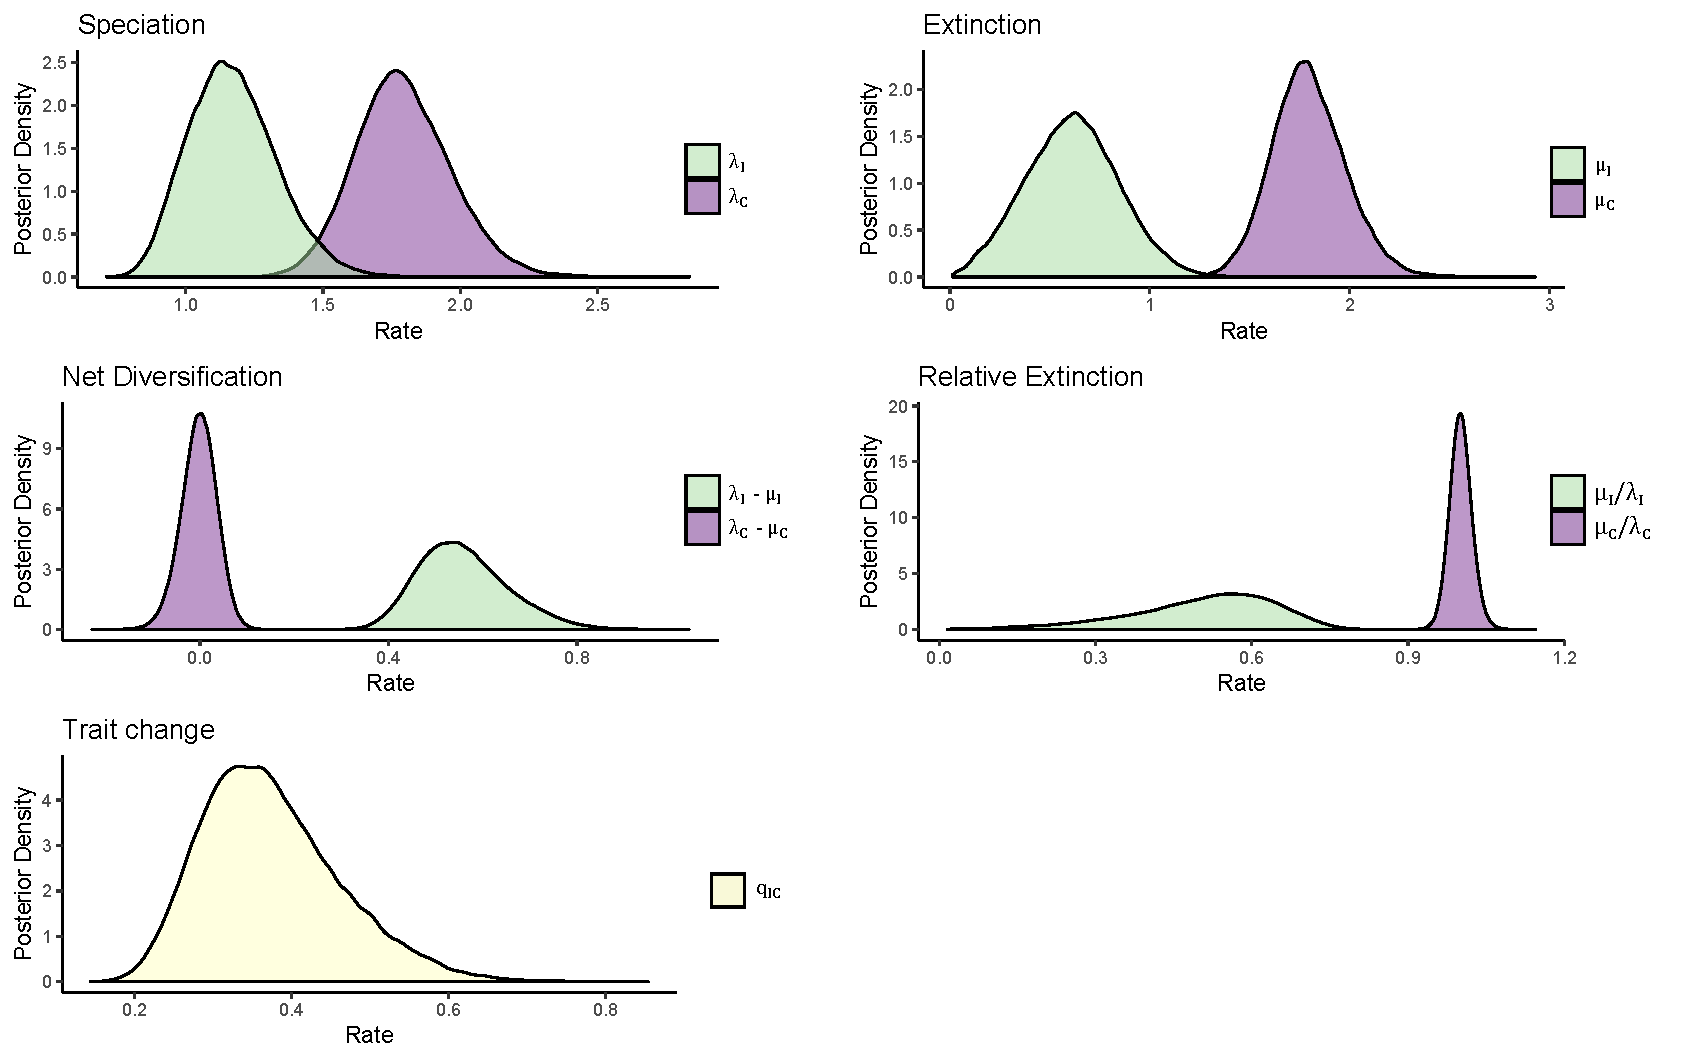
\includegraphics[width=\textwidth]{bisseSIposteriordist.pdf}
\caption{Posterior distribution for each of the parameters in the I/C breeding system model} % XXX
\label{suppfigure:IC}
\end{suppfigure}

\begin{suppfigure}
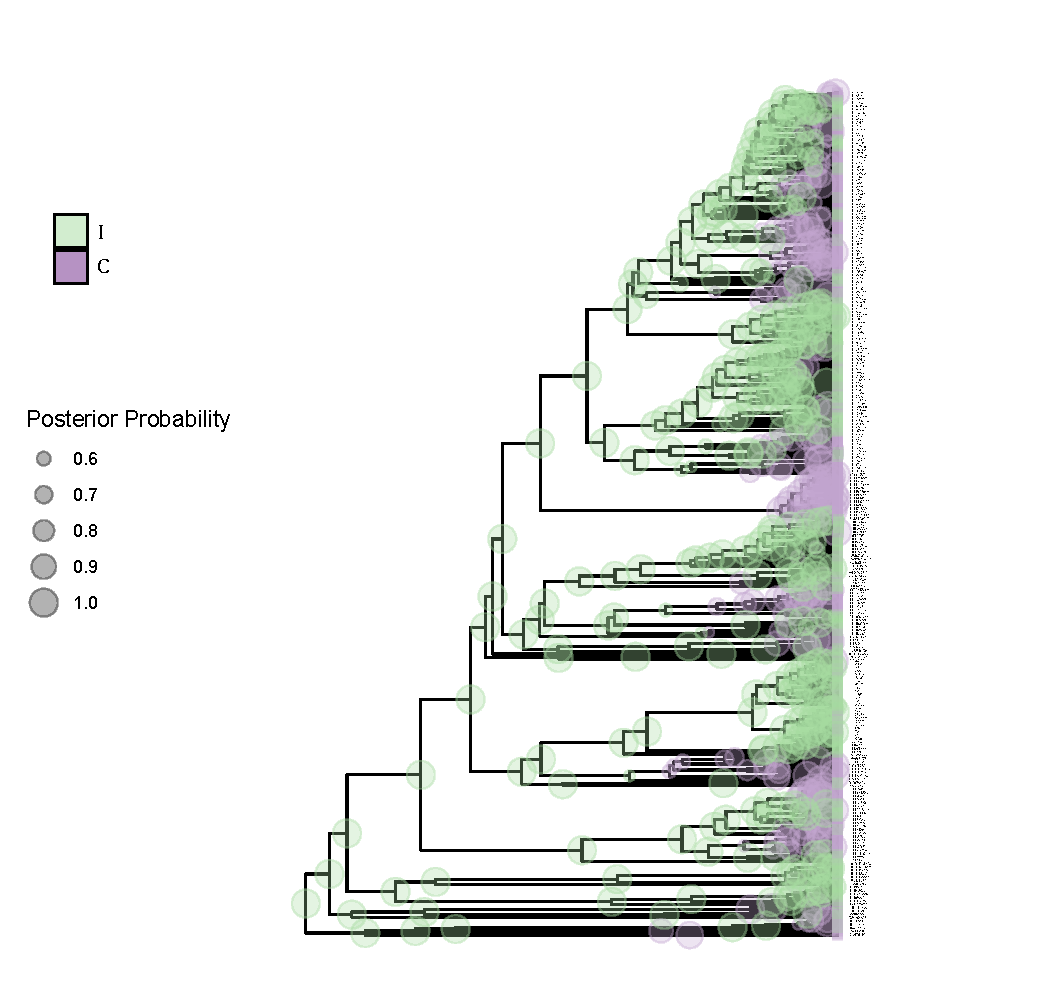
\includegraphics[width=\textwidth]{asrIC.pdf}
\caption{Ancestral state reconstruction showing the maximum a posteriori for each node in the I/C breeding system model} % XXX
\label{suppfigure:ICasr}
\end{suppfigure}

\begin{suppfigure}
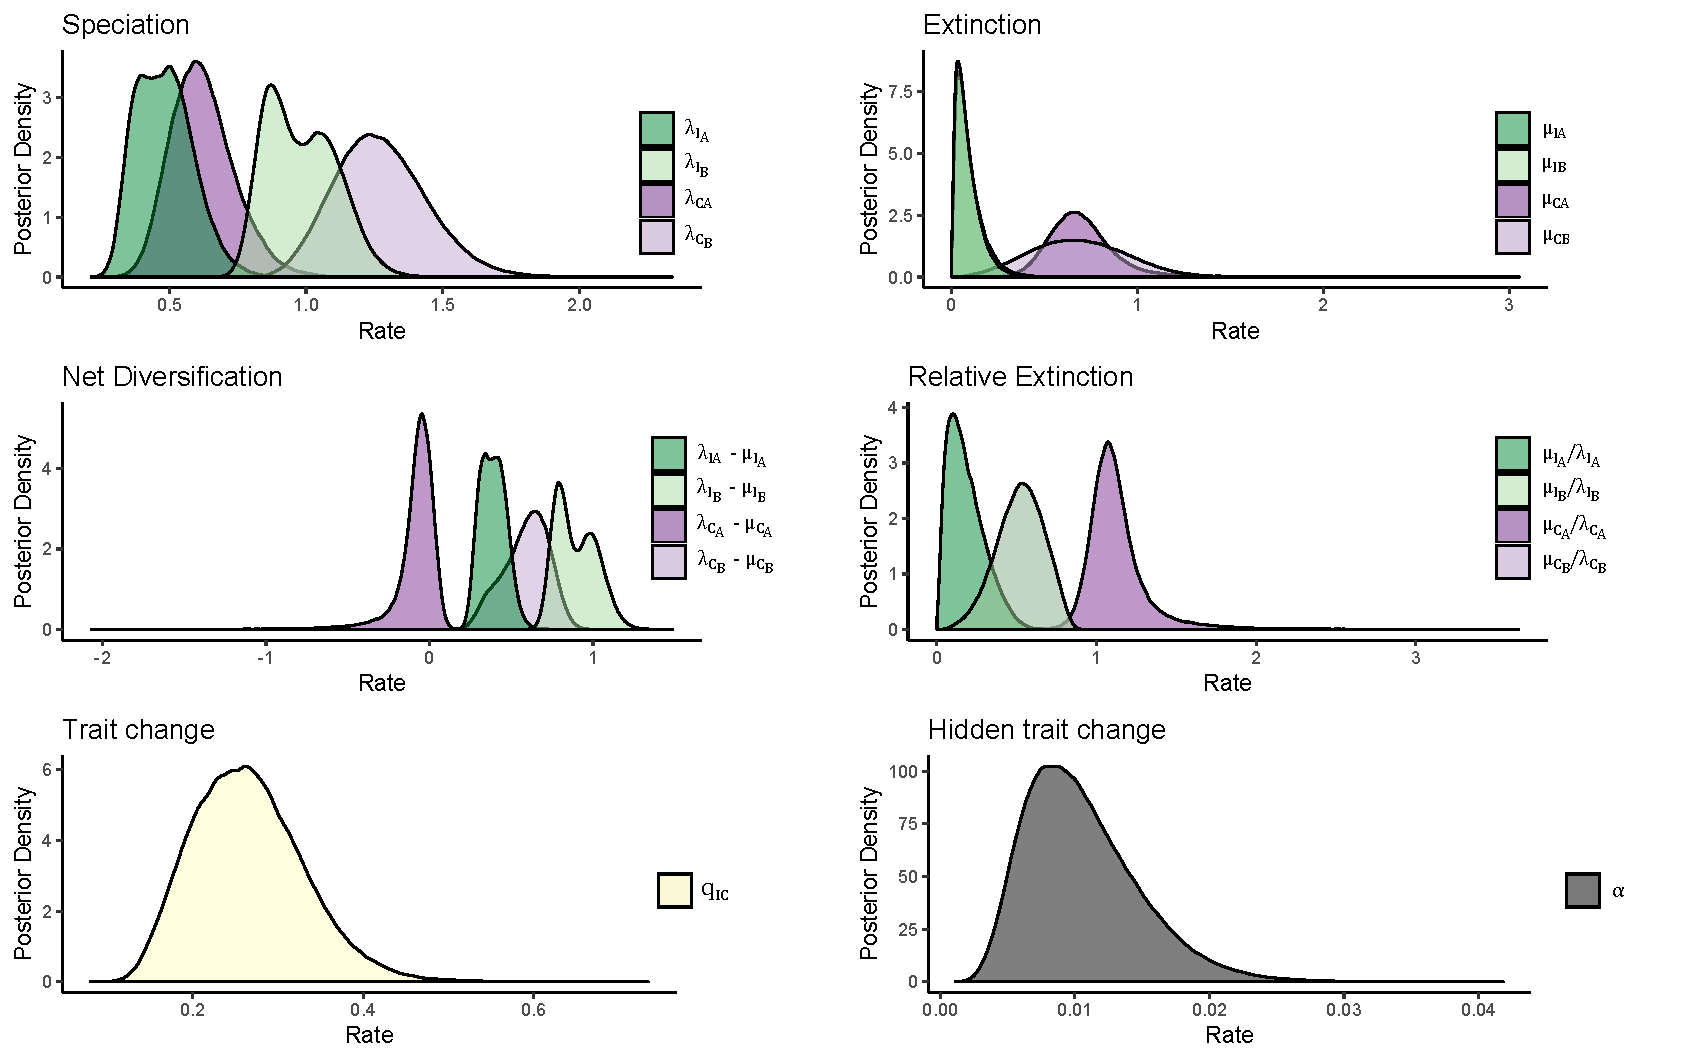
\includegraphics[width=\textwidth]{hisseSInoretposteriordist.pdf}
\caption{Posterior distribution for each of the parameters in the I/C+A/B, breeding system model} % XXX
\label{suppfigure:ICAB}
\end{suppfigure}

\begin{suppfigure}
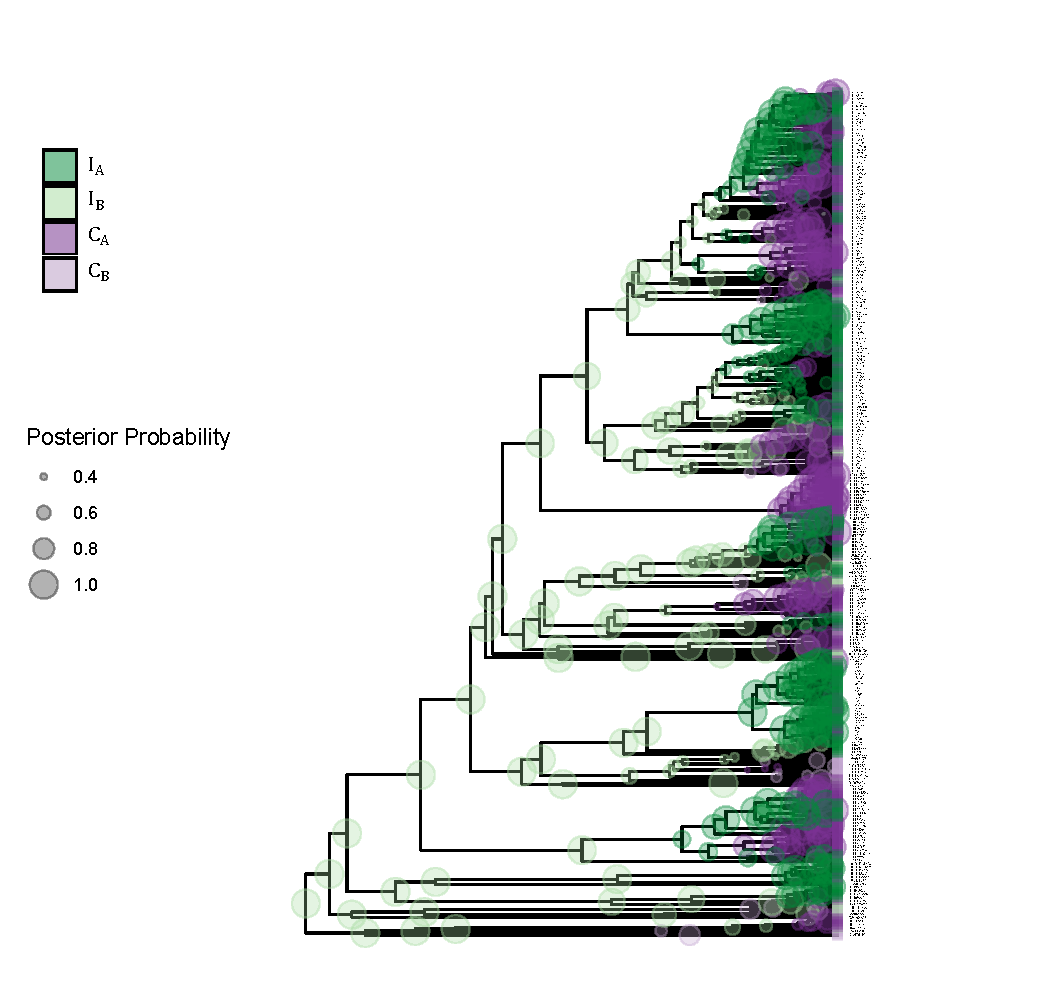
\includegraphics[width=\textwidth]{asrICAB.pdf}
\caption{Ancestral state reconstruction showing the maximum a posteriori for each node in the I/C+A/B breeding system model} % XXX
\label{suppfigure:ICABasr}
\end{suppfigure}

\begin{suppfigure}
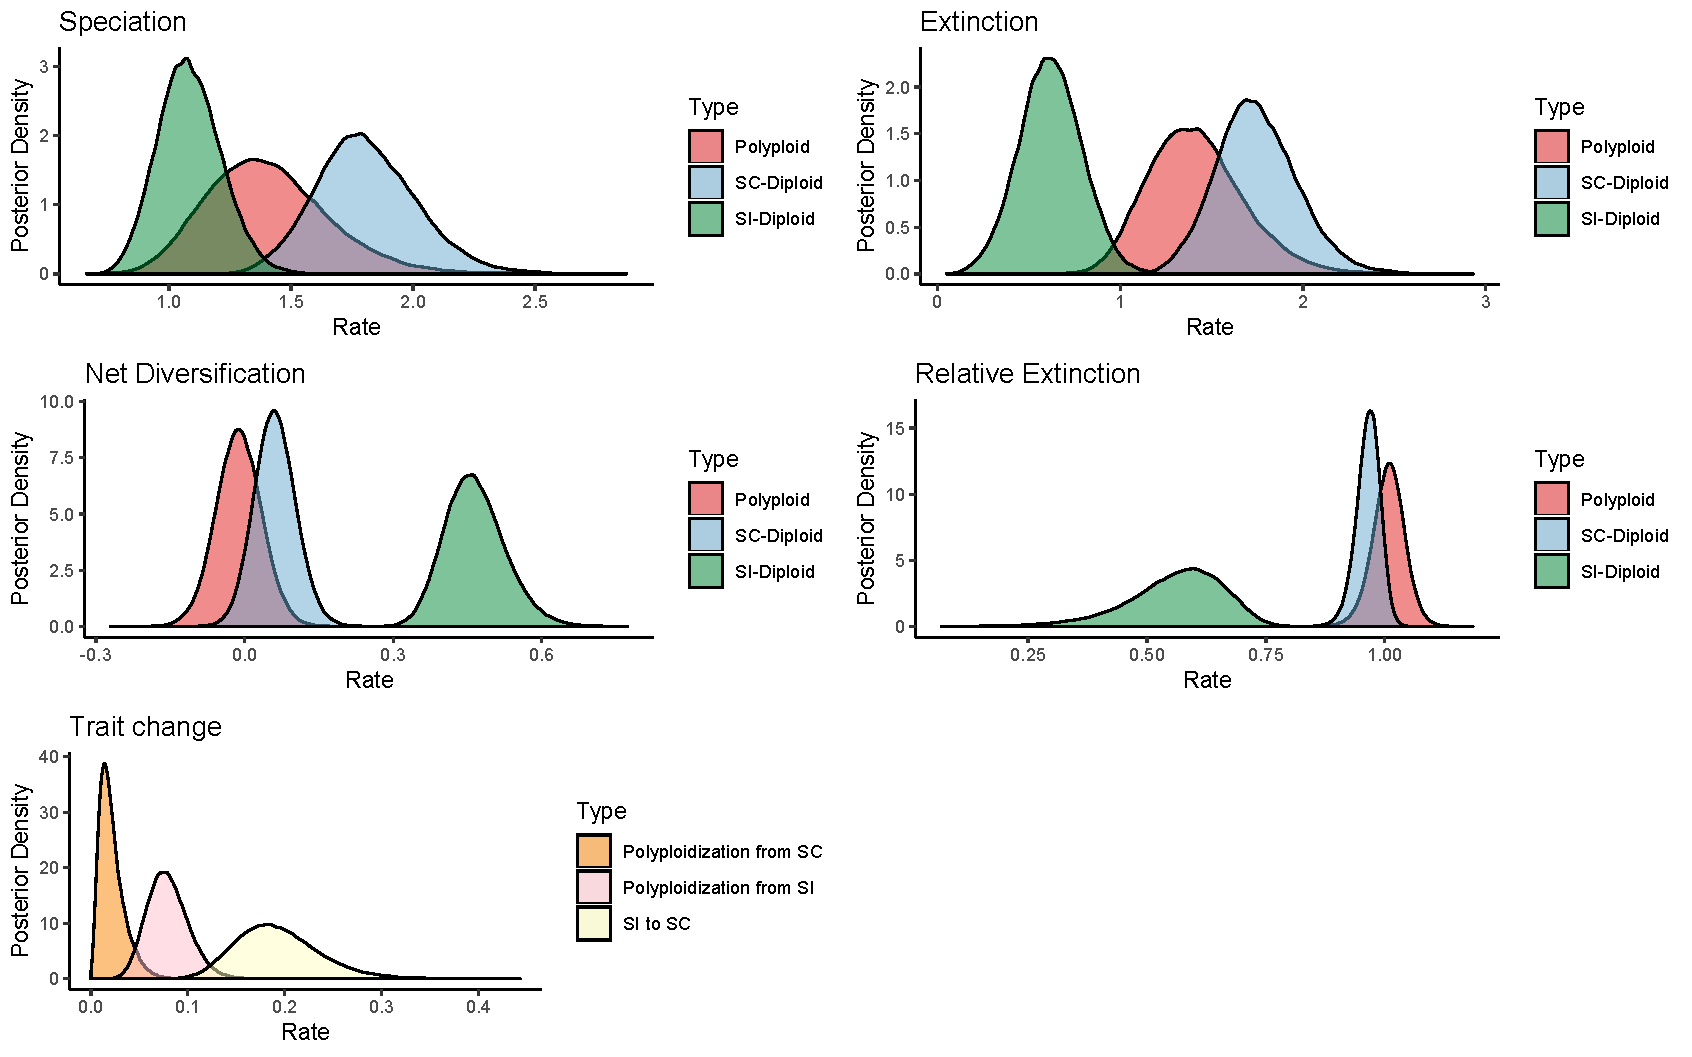
\includegraphics[width=\textwidth]{musseDPSInodipposteriordist.pdf}
\caption{Posterior distribution for each of the parameters in the ID/CD/CP ploidy and breeding system model} % XXX
\label{suppfigure:IDCDCPnodip}
\end{suppfigure}

\begin{suppfigure}
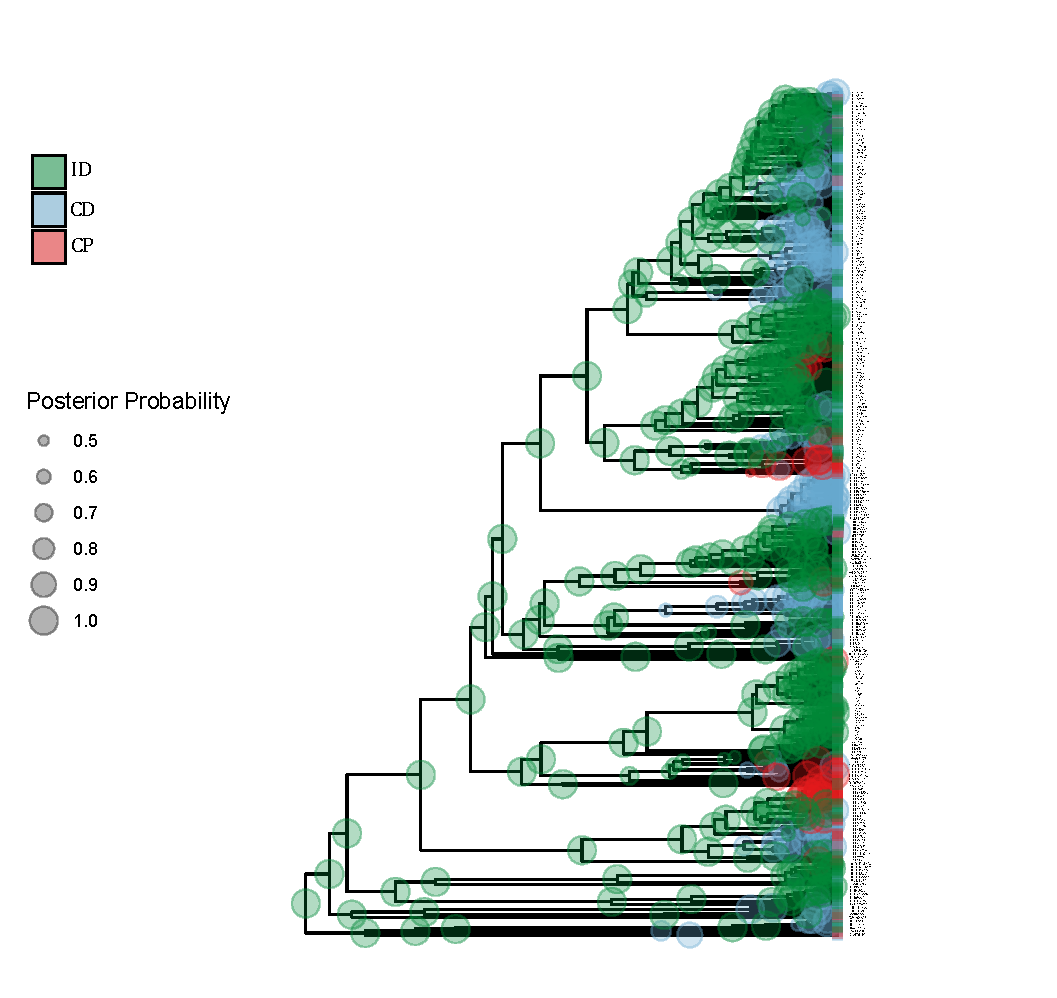
\includegraphics[width=\textwidth]{asrIDCDCP.pdf}
\caption{Ancestral state reconstruction showing the maximum a posteriori for each node in the ID/CD/CP ploidy and breeding system model} % XXX
\label{suppfigure:IDCDCPnodipasr}
\end{suppfigure}

\begin{suppfigure}
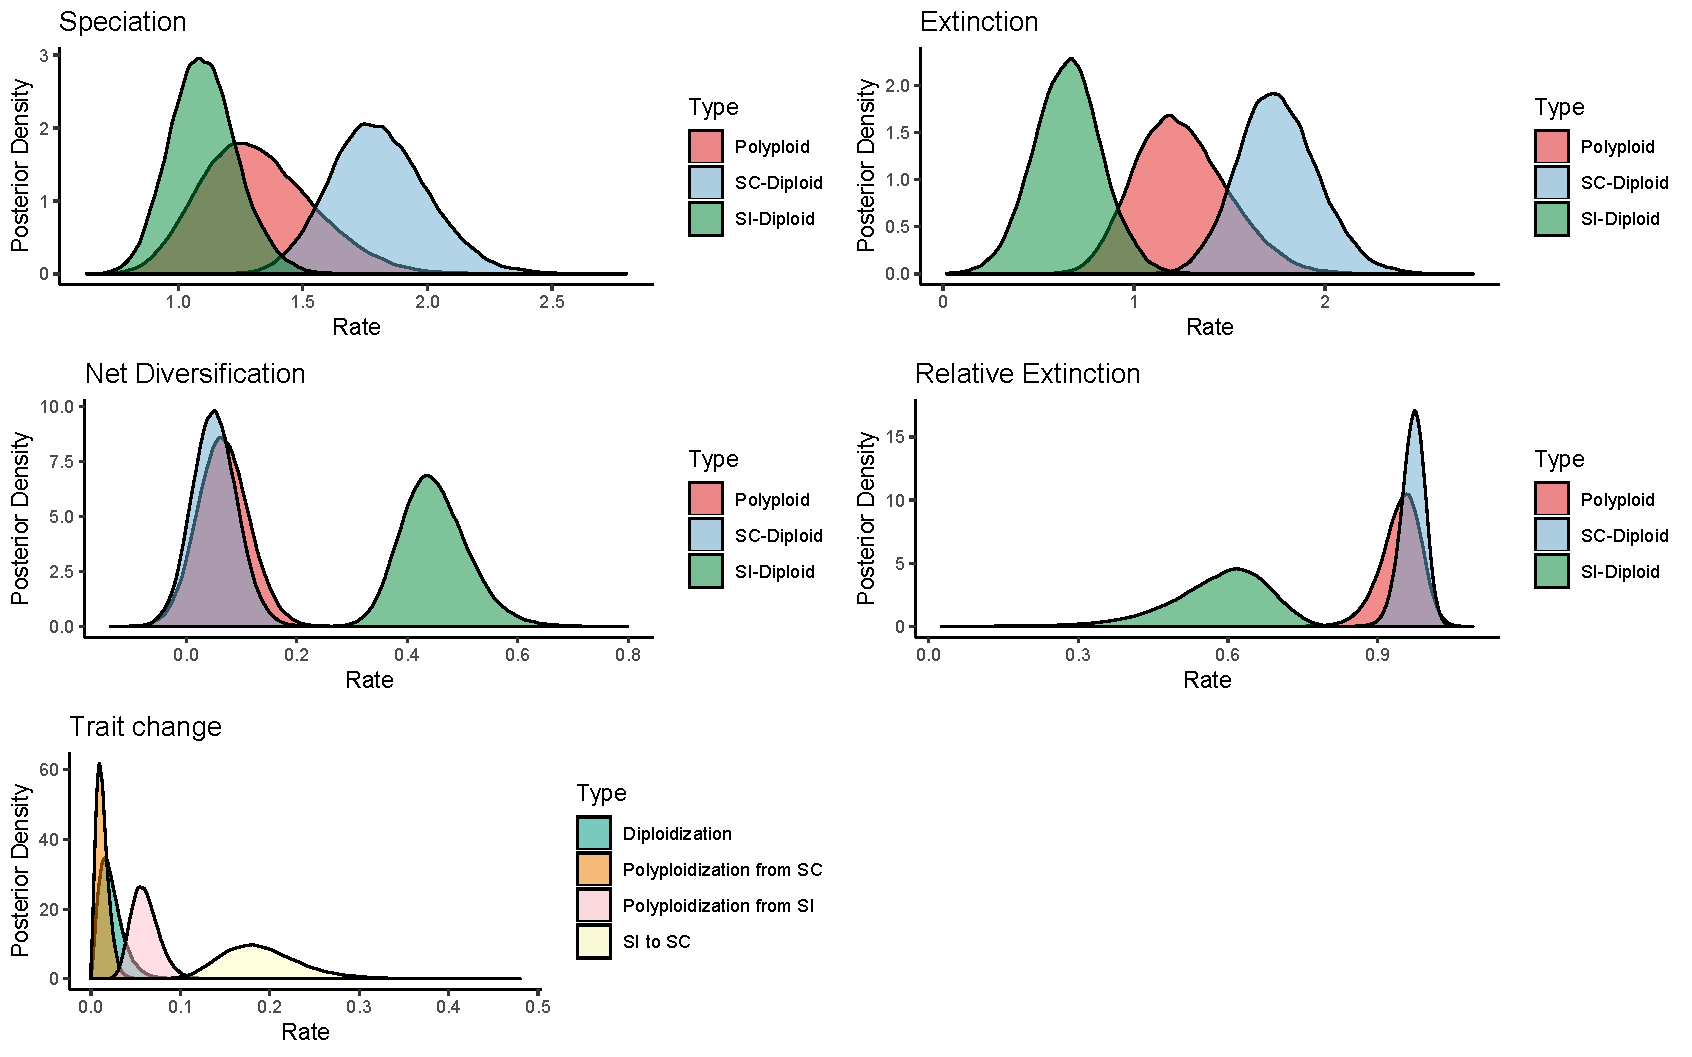
\includegraphics[width=\textwidth]{musseDPSIposteriordist.pdf}
\caption{Posterior distribution for each of the parameters in the ID/CD/CP+$\delta$, polyploidy and breeding system model} % XXX
\label{suppfigure:IDCDCP}
\end{suppfigure}

\begin{suppfigure}
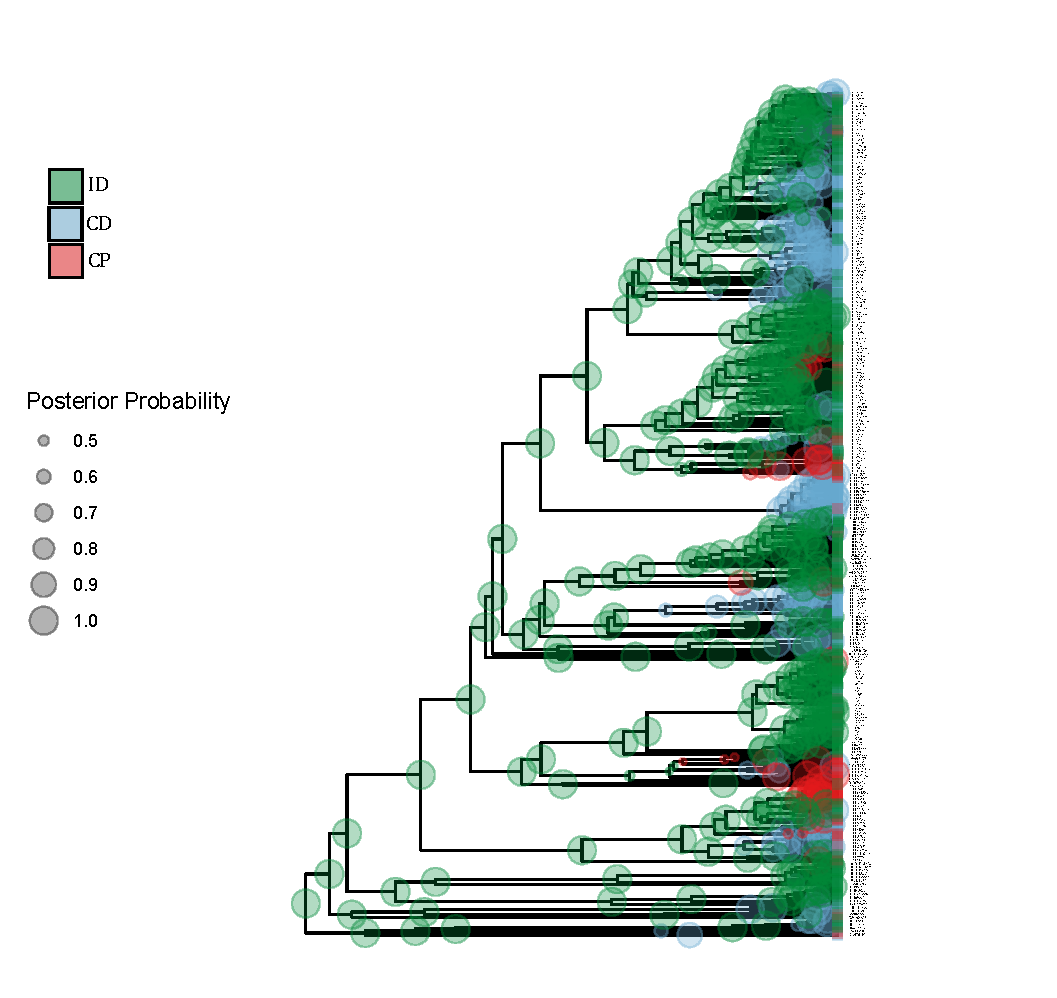
\includegraphics[width=\textwidth]{asrIDCDCPdelta.pdf}
\caption{Ancestral state reconstruction showing the maximum a posteriori for each node in the ID/CD/CP+$\delta$ ploidy and breeding system model} % XXX
\label{suppfigure:IDCDCPasr}
\end{suppfigure}


\begin{suppfigure}
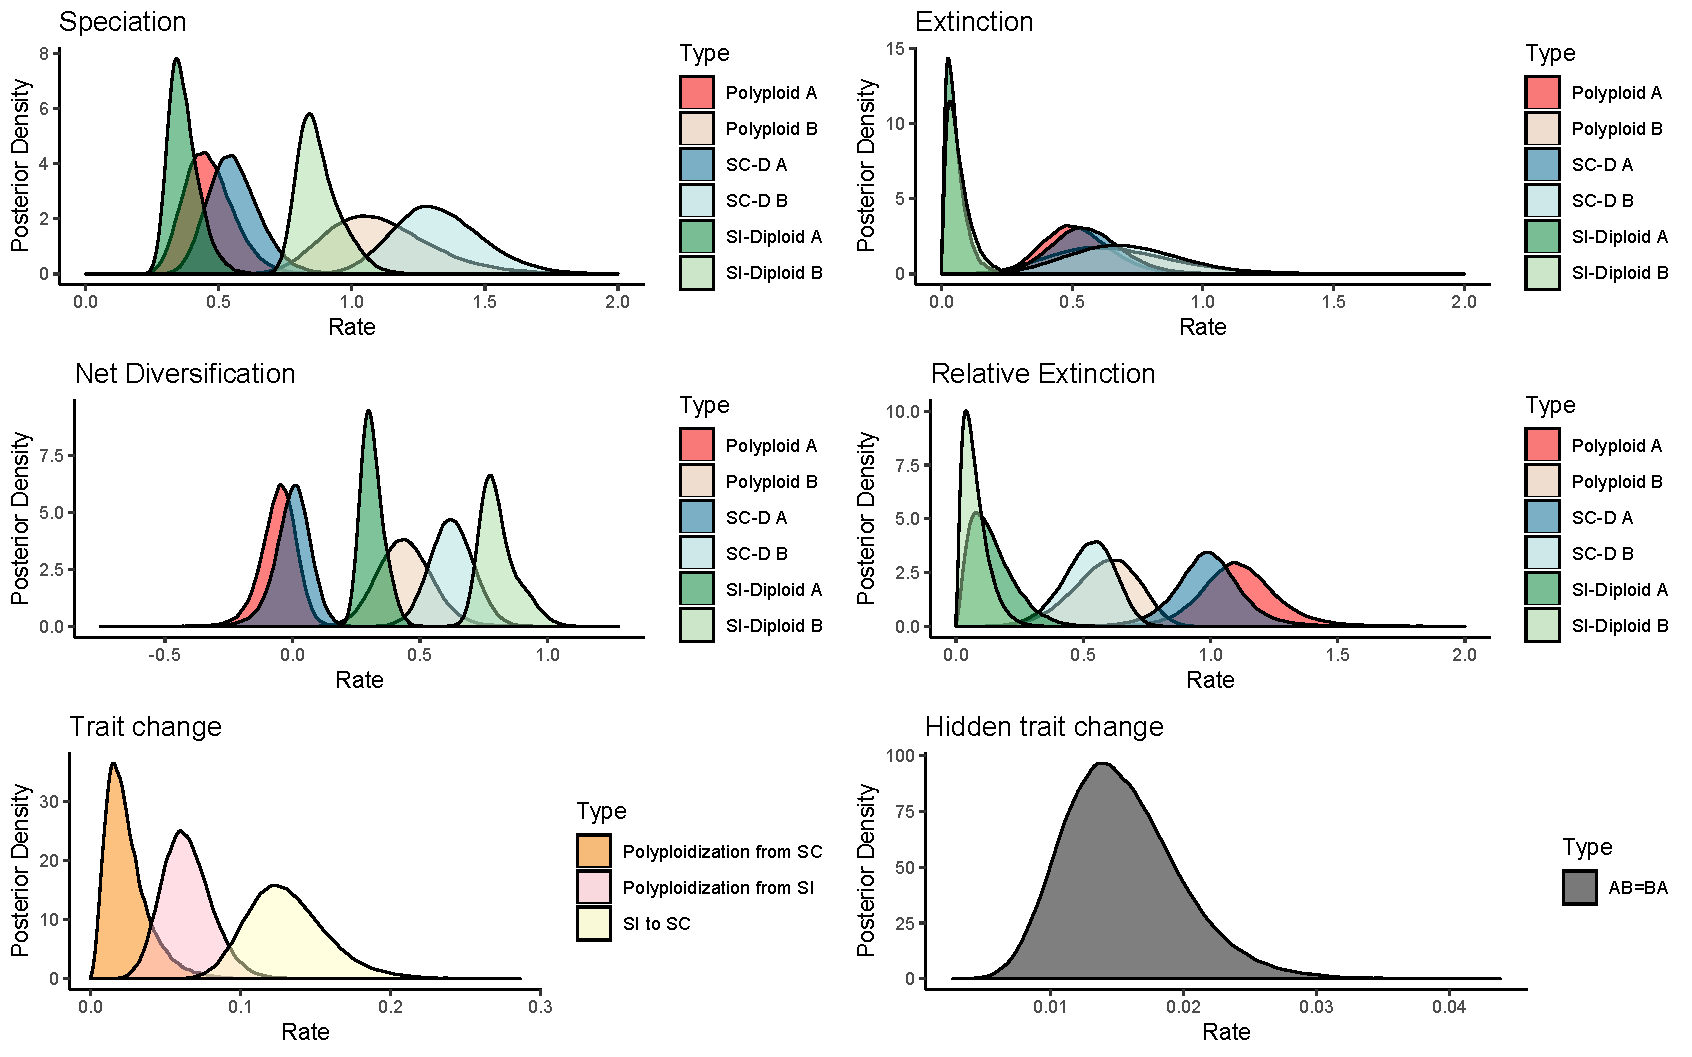
\includegraphics[width=\textwidth]{muhisseDPSInodipposteriordist.pdf}
\caption{Posterior distribution for each of the parameters in the ID/CD/CP+A/B polyploidy and breeding system model} % XXX
\label{suppfigure:IDCDCPnodipAB}
\end{suppfigure}

\begin{suppfigure}
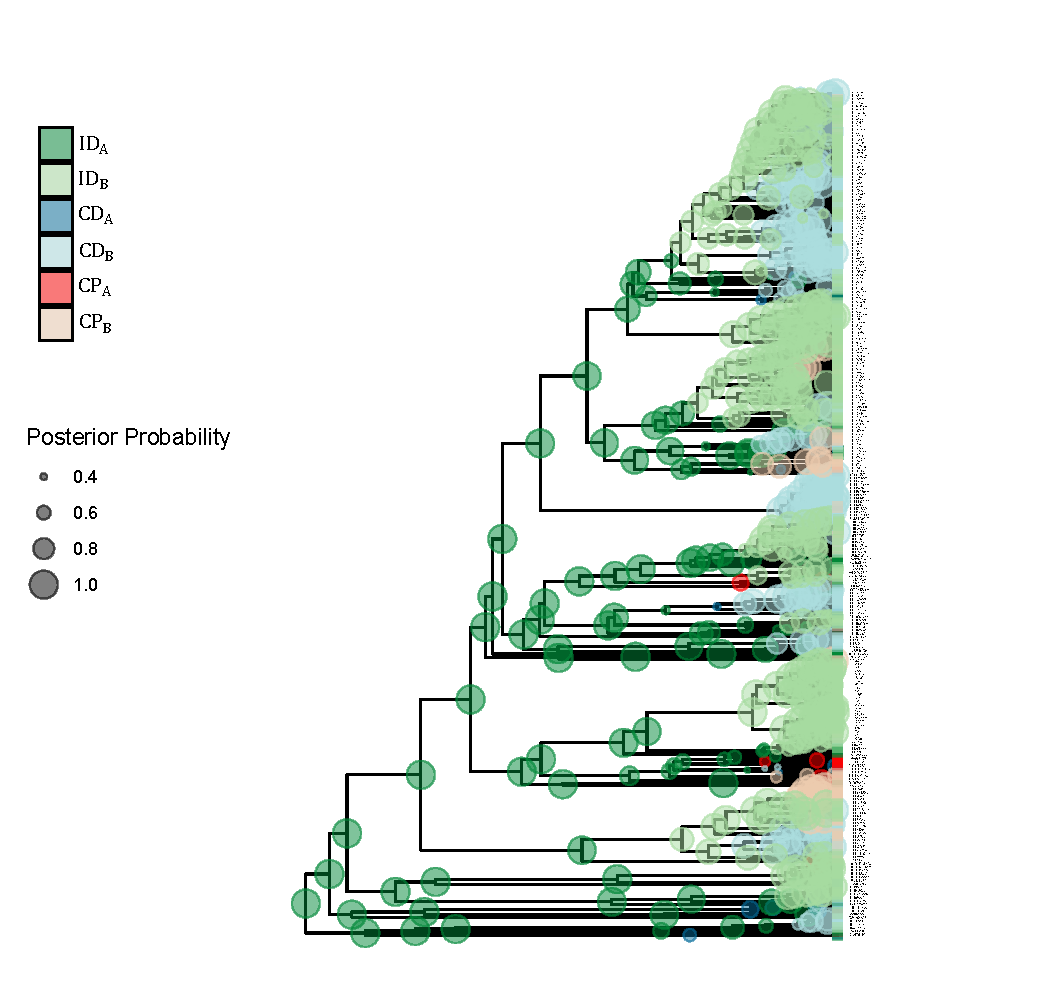
\includegraphics[width=\textwidth]{asrIDCDCPAB.pdf}
\caption{Ancestral state reconstruction showing the maximum a posteriori for each node in the ID/CD/CP+A/B polyploidy and breeding system model} % XXX
\label{suppfigure:IDCDCPnodipABasr}
\end{suppfigure}

\begin{suppfigure}
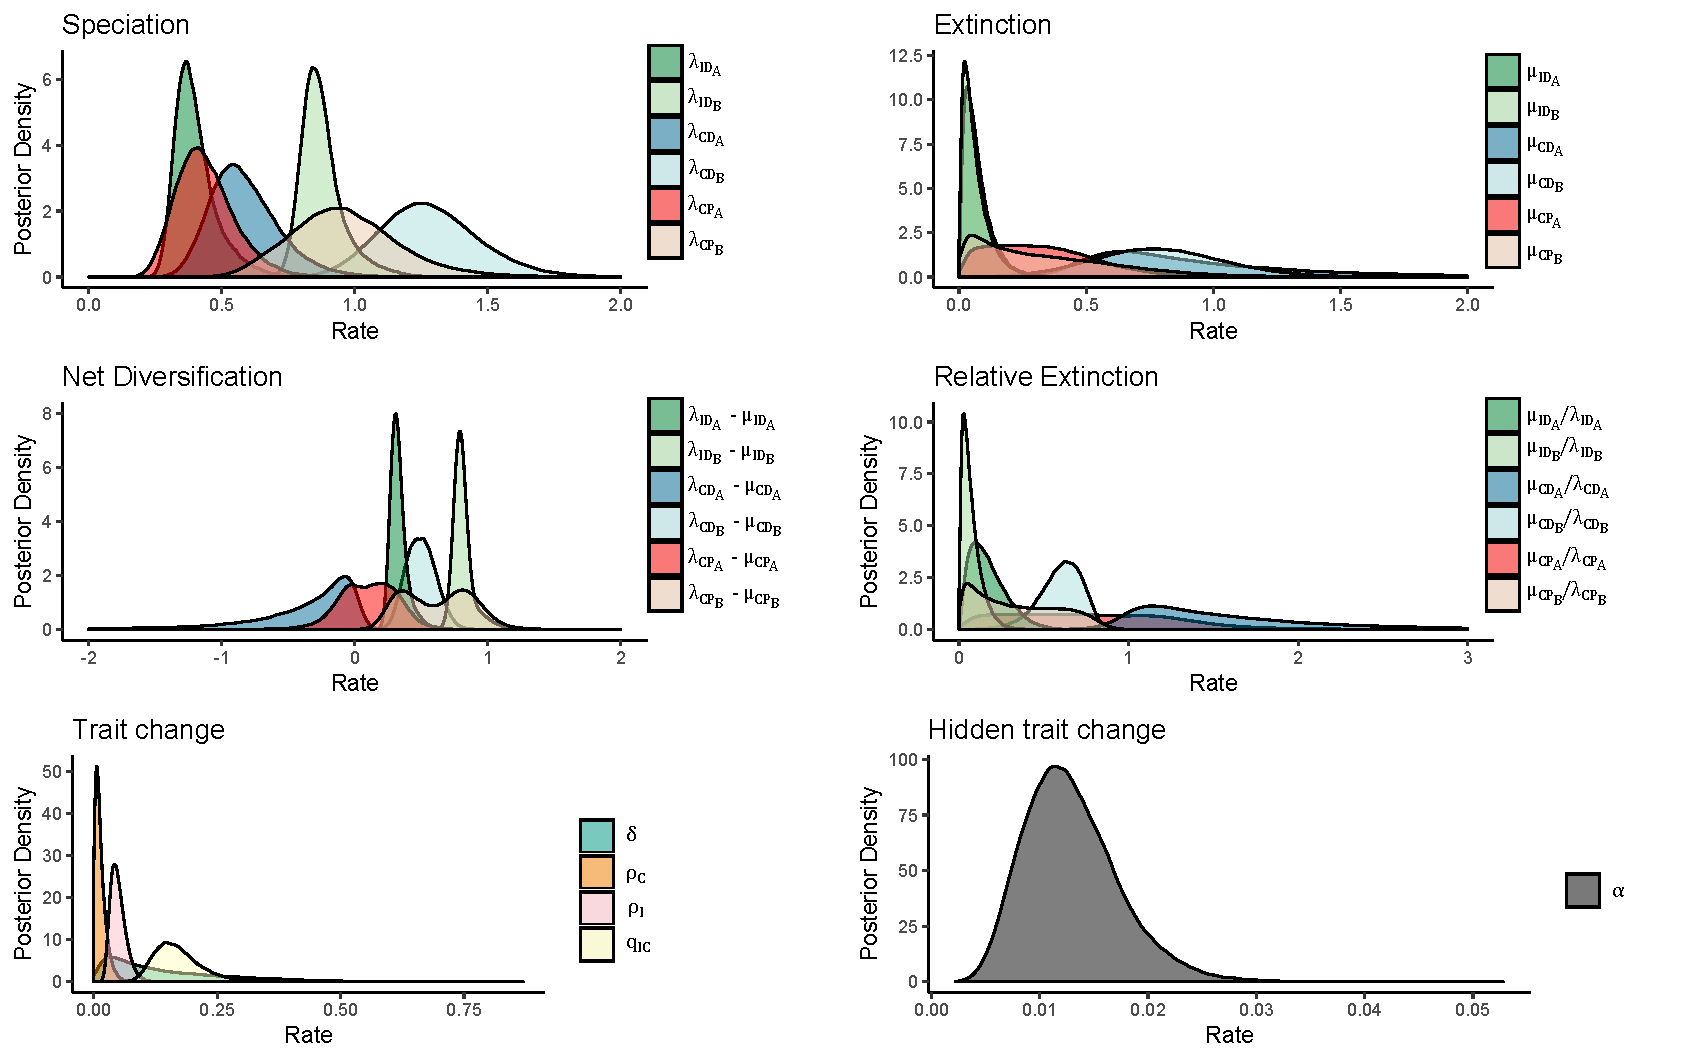
\includegraphics[width=\textwidth]{muhisseDPSIposteriordist.pdf}
\caption{Posterior distribution for each of the parameters in the ID/CD/CP+$\delta$+A/B, polyploidy and breeding system model} % XXX
\label{suppfigure:IDCDCPAB}
\end{suppfigure}

\begin{suppfigure}
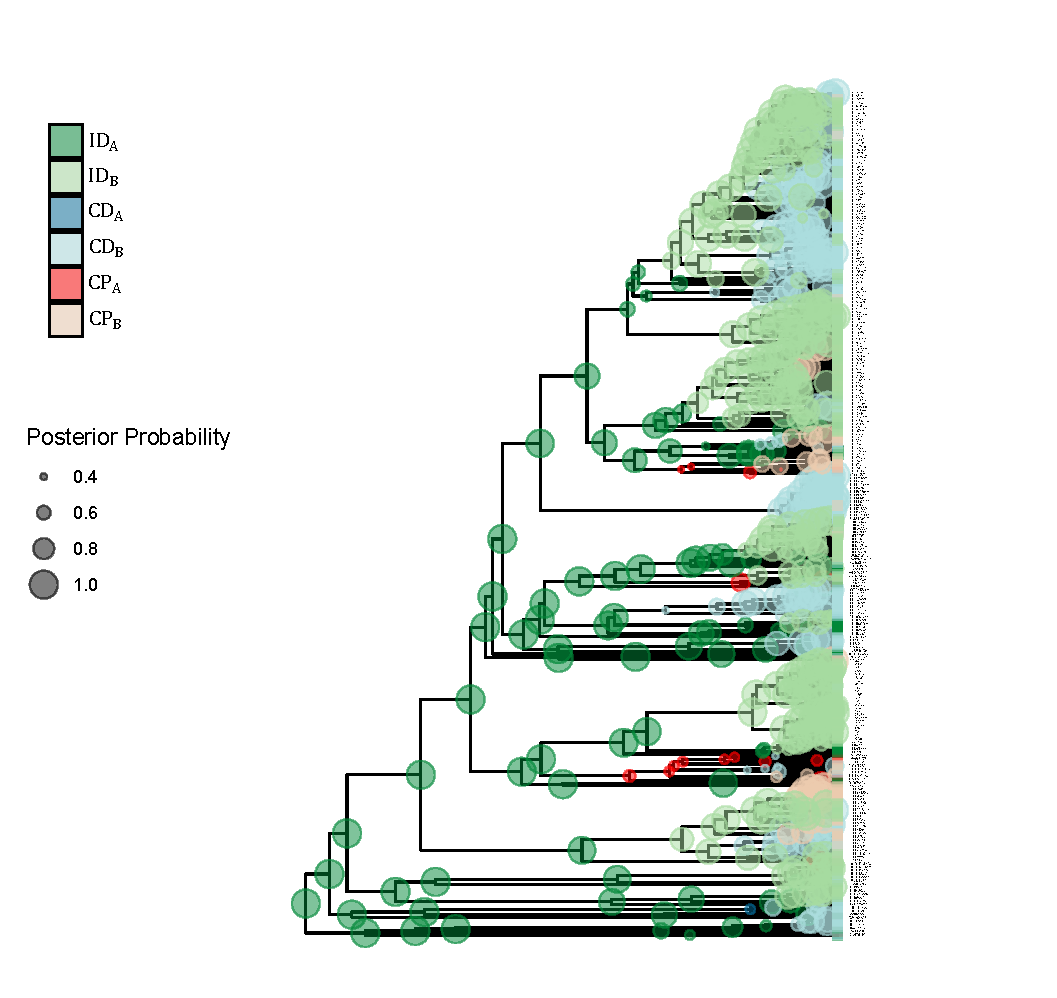
\includegraphics[width=\textwidth]{asrIDCDCPdeltaAB.pdf}
\caption{Ancestral state reconstruction showing the maximum a posteriori for each node in the ID/CD/CP+$\delta$+A/B, polyploidy and breeding system model} % XXX
\label{suppfigure:IDCDCPABasr}
\end{suppfigure}
